\documentclass[oneside,english]{book}
\usepackage[T1]{fontenc}
%% DK DK we do not accept accented letters, use the old LaTeX syntax
%% DK DK for them instead: \'e \`e  \"e \^e and so on.
%% DK DK \usepackage[latin1]{inputenc}
\usepackage[letterpaper]{geometry}
\geometry{verbose,tmargin=1in,bmargin=1in,lmargin=1in,rmargin=1in}

% table of contents and numbering
\usepackage{tocbibind}
\setcounter{secnumdepth}{3}
\setcounter{tocdepth}{3}

\usepackage{babel}
\usepackage{float}
\usepackage{textcomp}
\usepackage{amsmath}
\usepackage{amssymb}

\IfFileExists{url.sty}{\usepackage{url}}
                      {\newcommand{\url}{\texttt}}

% biblio
\usepackage[authoryear]{natbib}
% biblio GJI
\bibliographystyle{abbrvnat}

% fonts
\usepackage{times}

% figures
\usepackage{graphicx}

% we are running pdflatex, so convert .eps files to .pdf
\usepackage{epstopdf}

% colors to show the corrections
\usepackage[dvipsnames,usenames]{xcolor}
\definecolor{light-gray}{rgb}{0.7,0.7,0.7}
\definecolor{dark-gray}{rgb}{0.1,0.1,0.3}
\definecolor{light-blue}{rgb}{0.7,0.7,0.9}
\definecolor{dark-blue}{rgb}{0.2,0.2,0.5}

% create thumbnails
%\usepackage[pdftex]{thumbpdf}

% hyperlinks to sections and references
\usepackage[pdftex]{hyperref}
% more options
\hypersetup{
  bookmarks=true,
  bookmarksnumbered=true,
  pdfpagemode=UseNone,
  pdfstartview=FitH,
  pdfpagelayout=SinglePage,
  pdfborder={0 0 0},
  colorlinks=true,      % color links
  citecolor=dark-gray,  % citation links
  filecolor=dark-gray,  % file links
  linkcolor=dark-gray,  % internal link (rgb values)
  urlcolor=dark-blue    % external weblinks
}

% create thumbnails
%\usepackage[pdftex]{thumbpdf}

\usepackage{enumitem}

\makeatletter

% BibTeX logo
\newcommand{\BibTeX}{{\rm B\kern-.05em{\sc i\kern-.025em b}\kern-.08em{T}\kern-.1667em\lower.7ex\hbox{E}\kern-.125emX}}

%%%%%%%%%%%%%%%%%%%%%%%%%%%%%% User specified LaTeX commands.

% hyperlinks to sections and references
\newcommand{\urlwithparentheses}[1]{(\url{#1})}

\newcommand{\toall}[1]{\textbf{*** All: #1 ***}}
\newcommand{\tojeroen}[1]{\textbf{*** Jeroen: #1 ***}}
\newcommand{\tobrian}[1]{\textbf{*** Brian: #1 ***}}
\newcommand{\tovala}[1]{\textbf{*** Vala: #1 ***}}
\newcommand{\tovalabrian}[1]{\textbf{*** Vala \& Brian: #1 ***}}
\newcommand{\tovalaqinya}[1]{\textbf{*** Vala \& Qinya: #1 ***}}
\newcommand{\toqinya}[1]{\textbf{*** Qinya: #1 ***}}
\newcommand{\tomin}[1]{\textbf{*** Min: #1 ***}}
\newcommand{\toalessia}[1]{\textbf{*** Alessia: #1 ***}}
\newcommand{\todimitri}[1]{\textbf{*** Dimitri: #1 ***}}

% colors to show the corrections
\newcommand{\red}[1]{\textbf{\textcolor{Red}{#1}}}
\newcommand{\blue}[1]{\textbf{\textcolor{Blue}{#1}}}
\newcommand{\cyan}[1]{\textbf{\textcolor{Cyan}{#1}}}
\newcommand{\green}[1]{\textbf{\textcolor{Green}{#1}}}
\newcommand{\magenta}[1]{\textbf{\textcolor{Magenta}{#1}}}
\newcommand{\orange}[1]{\textbf{\textcolor{Orange}{#1}}}

\makeatother

%%%%%%%%%%%%%%%%%%%%%%%%%%%%%% Start of document.

\begin{document}

%%%%%%%%%%%%%%%%%%%%%%%%%%%%%%%%%%%%%%%%%%%%%%%%%
%% TITLE page
%%%%%%%%%%%%%%%%%%%%%%%%%%%%%%%%%%%%%%%%%%%%%%%%%
\newgeometry{margin=0pt}
\thispagestyle{empty}
\vspace*{\fill}
\begingroup
\centering
\makebox[\textwidth]{%
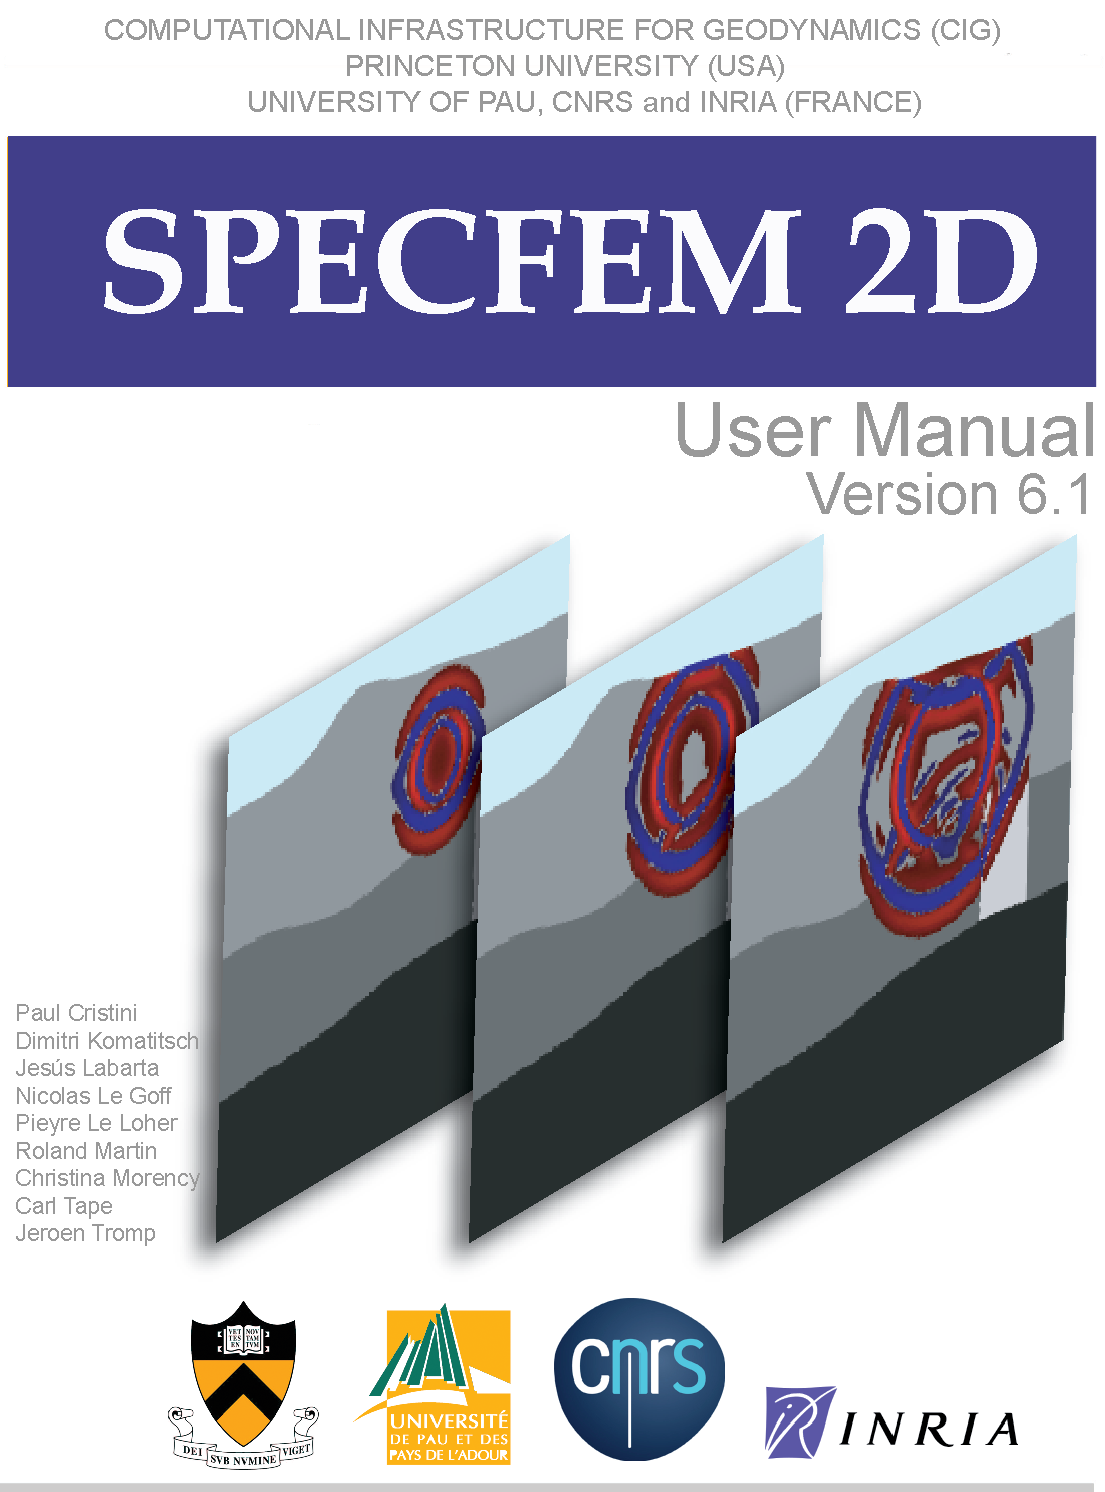
\includegraphics[width=0.83\paperwidth]{figures/specfem_2d-cover.pdf}
}
\endgroup
\vspace*{\fill}
\restoregeometry

% Inner Title Page
\title{\textbf{SPECFEM2D}\\
\textbf{User Manual}}

\author{\copyright\ CNRS (France) and Princeton University (USA)\\
Version 7.0
}

% date of last edit
\date{\today}

\maketitle

%%%%%%%%%%%%%%%%%%%%%%%%%%%%%%%%%%%%%%%%%%%%%%%%%

\section*{Authors}

The SPECFEM2D package was first developed by Dimitri
Komatitsch and Jean-Pierre Vilotte at Institut de Physique du Globe
(IPGP) in Paris, France from 1995 to 1997 and then by Dimitri Komatitsch
at Harvard University (USA), Caltech (USA) and then CNRS and University of Pau (France) from 1998 to 2005.
The story started on April 4, 1995, when Prof. Yvon Maday from CNRS and University of Paris, France, gave a lecture to
Dimitri Komatitsch and Jean-Pierre Vilotte at IPG about the nice properties of the Legendre spectral-element method with diagonal mass matrix that he had used for
other equations. We are deeply indebted and thankful to him for that.
That followed a visit by Dimitri Komatitsch to OGS (Istituto Nazionale di Oceanografia e di Geofisica Sperimentale) in Trieste, Italy, in February 1995
to meet with G\'eza Seriani and Enrico Priolo, who introduced him to their 2D Chebyshev version of the spectral-element method with a non-diagonal mass matrix.
We are deeply indebted and thankful to them for that.\\

%%%%%%%% please do NOT merge the lines of the paragraph below, it makes it difficult to insert new names in alphabetical order; leave a single name per line
%%%%%%%% please do NOT merge the lines of the paragraph below, it makes it difficult to insert new names in alphabetical order; leave a single name per line
%%%%%%%% please do NOT merge the lines of the paragraph below, it makes it difficult to insert new names in alphabetical order; leave a single name per line
Since then it has been developed and maintained by a development team: in alphabetical order,
\'Etienne Bachmann,
Alexis Bottero,
Quentin Brissaud,
Paul Cristini,
Dimitri Komatitsch,
Jes\'us Labarta,
Nicolas Le Goff,
Pieyre Le Loher,
Qinya Liu,
Youshan Liu,
Roland Martin,
Ren\'e Matzen,
Christina Morency,
Masaru Nagaso,
Daniel Peter,
Carl Tape,
Jeroen Tromp,
Jean-Pierre Vilotte,
Zhinan Xie.\\

The code is released open-source under the GNU version 3 license, see the license at the end of this manual.



\newpage{}

\section*{Current and past main participants or main sponsors of the SPECFEM project (in no particular order)}
%
\begin{figure}[htbp]
\noindent \begin{centering}
\includegraphics[width=0.125\textwidth]{figures/logo_cnrs}\vspace*{2truemm}
\includegraphics[width=0.125\textwidth]{figures/logo_princeton}\vspace*{2truemm}
\includegraphics[width=0.15\textwidth]{figures/logo_aix_marseille_universite}\vspace*{0.02truemm}
\includegraphics[width=0.15\textwidth]{figures/logo_ETH}\vspace*{2truemm}
\includegraphics[width=0.12\textwidth]{figures/logo_CSC_China}\vspace*{0.02truemm}
\includegraphics[width=0.15\textwidth]{figures/logo_inria}\vspace*{2truemm}
\includegraphics[width=0.14\textwidth]{figures/logo_UPPA}
\par\end{centering}
%
\vspace*{-2truemm}
%
\noindent \begin{centering}
\includegraphics[width=0.15\textwidth]{figures/logo_NVIDIA}\vspace*{2truemm}
\includegraphics[width=0.125\textwidth]{figures/logo_IUF}\vspace*{2truemm}
\includegraphics[width=0.135\textwidth]{figures/logo_Caltech}\vspace*{2truemm}
\includegraphics[width=0.135\textwidth]{figures/logo_Harvard}\vspace*{2truemm}
\includegraphics[width=0.135\textwidth]{figures/logo_IPGP}\vspace*{2truemm}
\includegraphics[width=0.112\textwidth]{figures/logo_ANR}\vspace*{2truemm}
\includegraphics[width=0.112\textwidth]{figures/logo_NSF}\vspace*{2truemm}
\par\end{centering}
%
\vspace*{-2truemm}
%
\noindent \begin{centering}
\includegraphics[width=0.190\textwidth]{figures/logo_European_Union}\vspace*{2truemm}
\includegraphics[width=0.112\textwidth]{figures/logo_GENCI}\vspace*{2truemm}
\includegraphics[width=0.112\textwidth]{figures/logo_PRACE}\vspace*{2truemm}
\includegraphics[width=0.112\textwidth]{figures/logo_CINES}\vspace*{2truemm}
\includegraphics[width=0.130\textwidth]{figures/logo_Oak_Ridge}\vspace*{2truemm}
\hspace*{3mm}\includegraphics[width=0.130\textwidth]{figures/logo_fondation_Del_Duca}
\includegraphics[width=0.130\textwidth]{figures/logo_CIG}\vspace*{2truemm}
\par\end{centering}
%
\vspace*{-2truemm}
%
\noindent \begin{centering}
\includegraphics[width=0.112\textwidth]{figures/logo_University_of_Toronto}\vspace*{2truemm}
\includegraphics[width=0.109\textwidth]{figures/logo_INGV}\vspace*{2truemm}
\includegraphics[width=0.102\textwidth]{figures/logo_Univ_Toulouse}\vspace*{2truemm}
\includegraphics[width=0.112\textwidth]{figures/logo_TOTAL}\vspace*{2truemm}
\includegraphics[width=0.130\textwidth]{figures/logo_Fairbanks}\vspace*{2truemm}
\includegraphics[width=0.120\textwidth]{figures/logo_CINECA}\vspace*{2truemm}
\includegraphics[width=0.140\textwidth]{figures/logo_Intel_Exascale_Labs}\vspace*{2truemm}
\includegraphics[width=0.130\textwidth]{figures/logo_Maison_Simulation}
\par\end{centering}
\end{figure}




%%%%%%%%%%%%%%%%%%%%%%%%%%%%%%%%%%%%%%%%%%%%%%%%%
%% Table of contents
%%%%%%%%%%%%%%%%%%%%%%%%%%%%%%%%%%%%%%%%%%%%%%%%%

\newpage{}

\tableofcontents{}

%%%%%%%%%%%%%%%%%%%%%%%%%%%%%%%%%%%%%%%%%%%%%%%%%

%------------------------------------------------------------------------------------------------%

\chapter{Introduction}

%------------------------------------------------------------------------------------------------%

SPECFEM2D allows users to perform 2D and 2.5D (i.e., axisymmetric) simulations of
acoustic, elastic, viscoelastic, and poroelastic seismic wave propagation
as well as full waveform imaging (FWI) or adjoint tomography.\\

\red{In fluids,
%% DK DK removed that because gravity is implemented in SPECFEM3D but not in SPECFEM2D
% when gravity is turned off,
SPECFEM2D uses the classical linearized Euler equation; thus if you have sharp local variations of density in the fluid (highly heterogeneous fluids
in terms of density) or if density becomes extremely small in some regions of your model (e.g. for upper-atmosphere studies), before using the code please make sure the linearized Euler equation is a valid approximation in the case you want to study. For more details on that see e.g. \cite{COA2011}.}\\

The 2D spectral-element solver accommodates
regular and unstructured meshes, generated for example by Cubit
\urlwithparentheses{http://cubit.sandia.gov},
Gmsh \urlwithparentheses{http://geuz.org/gmsh}
or GiD \urlwithparentheses{http://www.gid.cimne.upc.es}.
Even mesh creation packages that generate triangles, for instance Delaunay-Voronoi triangulation codes, can be used because each triangle can then easily be decomposed into three quadrangles by linking the barycenter to the center of each edge; while this approach does not generate quadrangles of optimal quality, it can ease mesh creation in some situations and it has been shown that the spectral-element method can very accurately handle distorted mesh elements.\\

With version 7.0, the 2D spectral-element solver accommodates Convolution PML absorbing layers and well as higher-order time schemes
(4th order Runge-Kutta and LDDRK4-6).
Convolution or Auxiliary Differential Equation Perfectly Matched absorbing Layers (C-PML or ADE-PML)
are described in \cite{MaKoEz08,MaKoGe08,MaKo09,MaKoGeBr10,KoMa07}.\\

The solver has adjoint capabilities and can
calculate finite-frequency sensitivity kernels \citep{TrKoLi08,PeKoLuMaLeCaLeMaLiBlNiBaTr11} for acoustic,
(an)elastic, and poroelastic media. The package also considers 2D SH
and P-SV wave propagation. Finally, the solver can run
both in serial and in parallel. See SPECFEM2D
\urlwithparentheses{http://www.geodynamics.org/cig/software/packages/seismo/specfem2d}
for the source code.\\

The SEM is a continuous Galerkin technique \citep{TrKoLi08,PeKoLuMaLeCaLeMaLiBlNiBaTr11}, which can easily be made discontinuous \citep{BeMaPa94,Ch00,KoWoHu02,ChCaVi03,LaWaBe05,Kop06,WiStBuGh10,AcKo11}; it is then close to a particular case of the discontinuous Galerkin technique \citep{ReHi73,LeRa74,Arn82,JoPi86,BoMaHe91,FaRi99,HuHuRa99,CoKaSh00,GiHeWa02,RiWh03,MoRi05,GrScSc06,AiMoMu06,BeLaPi06,DuKa06,DeSeWh08,PuAmKa09,WiStBuGh10,DeSe10,EtChViGl10}, with optimized efficiency because of its tensorized basis functions \citep{WiStBuGh10,AcKo11}.
In particular, it can accurately handle very distorted mesh elements \citep{OlSe11}.\\

It has very good accuracy and convergence properties \citep{MaPa89,SePr94,DeFiMu02,Coh02,DeSe07,SeOl08,AiWa09,AiWa10,MeStTh12}.
The spectral element approach admits spectral rates of convergence and allows exploiting $hp$-convergence schemes.
It is also very well suited to parallel implementation on very large supercomputers \citep{KoTsChTr03,TsKoChTr03,KoLaMi08a,CaKoLaTiMiLeSnTr08,KoViCh10}
as well as on clusters of GPU accelerating graphics cards \citep{Kom11,MiKo10,KoMiEr09,KoErGoMi10}.
Tensor products inside each element can be optimized to reach very high efficiency \citep{DeFiMu02}, and mesh point and element numbering can be optimized to reduce processor cache misses and improve cache reuse \citep{KoLaMi08a}. The SEM can also handle triangular (in 2D) or tetrahedral (in 3D) elements \citep{WinBoyd96,TaWi00,KoMaTrTaWi01,Coh02,MeViSa06} as well as mixed meshes, although with increased cost and reduced accuracy in these elements, as in the discontinuous Galerkin method.\\

Note that in many geological models in the context of seismic wave propagation studies
(except for instance for fault dynamic rupture studies, in which very high frequencies or supershear rupture need to be modeled near the fault, see e.g. \cite{BeGlCrViPi07,BeGlCrVi09,PuAmKa09,TaCrEtViBeSa10})
a continuous formulation is sufficient because material property contrasts are not drastic and thus
conforming mesh doubling bricks can efficiently handle mesh size variations \citep{KoTr02a,KoLiTrSuStSh04,LeChLiKoHuTr08,LeChKoHuTr09,LeKoHuTr09}.\\

For a detailed introduction to the SEM as applied to regional
seismic wave propagation, please consult \citet{PeKoLuMaLeCaLeMaLiBlNiBaTr11,TrKoLi08,KoVi98,KoTr99,ChKoViCaVaFe07} and
in particular \citet{LeKoHuTr09,LeChKoHuTr09,LeChLiKoHuTr08,GoAmTaCaSmSaMaKo09,WiKoScTr04,KoLiTrSuStSh04}.
A detailed theoretical analysis of the dispersion
and stability properties of the SEM is available in \citet{Coh02}, \citet{DeSe07}, \citet{SeOl07}, \citet{SeOl08} and \citet{MeStTh12}.\\

The SEM was originally developed in computational fluid dynamics \citep{Pat84,MaPa89}
and has been successfully adapted to address problems in seismic wave propagation.
Early seismic wave propagation applications of the SEM, utilizing Legendre basis functions and a
perfectly diagonal mass matrix, include \cite{CoJoTo93}, \cite{Kom97},
\cite{FaMaPaQu97}, \cite{CaGa97}, \cite{KoVi98} and \cite{KoTr99},
whereas applications involving Chebyshev basis functions and a non-diagonal mass matrix
include \cite{SePr94}, \cite{PrCaSe94} and \cite{SePrPr95}.
In the Legendre version that we use in SPECFEM the mass matrix is purposely slightly inexact but diagonal (but can be made exact if needed, see \cite{Teu15}),
while in the Chebyshev version it is exact but non diagonal.\\

\red{Beware that, in a spectral-element method, some spurious modes (that have some similarities with classical so-called "Hourglass modes" in finite-element techniques,
although in the SEM they are not zero-energy modes) can appear in some (but not all) cases in the spectral element in which the source is located.
Fortunately, they do not propagate away from the source element.
However, this means that if you put a receiver in the same spectral element as a source, the recorded signals may in some cases be wrong, typically exhibiting some spurious
oscillations, which are often even non causal.
If that is the case, an easy option is to slightly change the mesh in the source region in order to get rid of these Hourglass-like spurious modes,
as explained in \cite{DuLiScGa14}, in which this phenomenon is described in details, and in which practical solutions to avoid it are suggested.}\\

All SPECFEM2D software is written in Fortran2003 with full portability
in mind, and conforms strictly to the Fortran2003 standard. It uses
no obsolete or obsolescent features of Fortran. The package uses
parallel programming based upon the Message Passing Interface (MPI)
\citep{GrLuSk94,Pac97}.\\

This new release of the code includes support for GPU graphics card acceleration \citep{Kom11,MiKo10,KoMiEr09,KoErGoMi10}.\\

The code uses the plane strain convention when the standard P-SV equation case is used, i.e.,
the off-plane strain $\epsilon_{zz}$ is zero by definition of the plane strain convention but the off-plane stress $\sigma_{zz}$ is not equal to zero,
one has $\sigma_{zz} = \lambda (\epsilon_{xx} + \epsilon_{yy})$.
This implies, as in any plain strain software package, that the P-SV source is a line source along the direction perpendicular to the plane (see file
discussion\_of\_2D\_sources\_and\_approximations\_from\_Pilant\_1979.pdf for more details).

%------------------------------------------------------------------------------------------------%
\section{Citation}
%------------------------------------------------------------------------------------------------%

You can find all the references below in \BibTeX format in file \texttt{doc/USER\_MANUAL/bibliography.bib}.\\

If you use this code for your own research, please cite at least one article
written by the developers of the package, for instance:
%
\begin{itemize}
\item \cite{TrKoLi08},
\item \cite{PeKoLuMaLeCaLeMaLiBlNiBaTr11},
\item \cite{VaCaSaKoVi99},
\item \cite{LeChKoHuTr09},
\item \cite{LeChLiKoHuTr08},
\item \cite{LeKoHuTr09},
\item \cite{KoErGoMi10},
\item \cite{KoMiEr09},
\item \cite{LiPoKoTr04},
\item \cite{ChKoViCaVaFe07},
\item \cite{KoVi98},
\item \cite{KoTr99},
\item \cite{KoLiTrSuStSh04},
\item \cite{MoTr08},
\item \cite{BlKoChLoXi16},
\item and/or other articles from \url{http://komatitsch.free.fr/publications.html}.
\end{itemize}
%
If you use the C-PML absorbing layer capabilities of the code, please cite at least one article
written by the developers of the package, for instance:
%
\begin{itemize}
\item \cite{XiKoMaMa14},
\item \cite{XiMaCrKoMa16}.
\end{itemize}
%
If you use the UNDO\_ATTENUATION option of the code in order to produce full anelastic/viscoelastic sensitivity kernels, please cite at least one article
written by the developers of the package, for instance (and in particular):
%
\begin{itemize}
\item \cite{KoXiBoPeSaLiTr16}.
\end{itemize}
%
More generally, if you use the attenuation (anelastic/viscoelastic) capabilities of the code, please cite at least one article
written by the developers of the package, for instance:
%
\begin{itemize}
\item \cite{KoXiBoPeSaLiTr16},
\item \cite{BlKoChLoXi16}.
\end{itemize}
%
If you use the kernel capabilities of the code, please cite at least one article
written by the developers of the package, for instance:
%
\begin{itemize}
\item \cite{TrKoLi08},
\item \cite{PeKoLuMaLeCaLeMaLiBlNiBaTr11},
\item \cite{LiTr06},
\item \cite{MoLuTr09}.
\end{itemize}
%
If you use the SCOTCH / CUBIT non-structured capabilities, please cite:
%
\begin{itemize}
\item \cite{MaKoBlLe08}.
\end{itemize}
%
If you use axisymmetric geometries please also cite:
\begin{itemize}
 \item \cite{BoCrKoAs16}
\end{itemize}
%
The corresponding Bib\TeX{} entries may be found
in file \texttt{doc/USER\_MANUAL/bibliography.bib}.



%------------------------------------------------------------------------------------------------%
\section{Support}
%------------------------------------------------------------------------------------------------%

This material is based upon work supported by the USA National Science
Foundation under Grants No. EAR-0406751 and EAR-0711177, by the French
CNRS, French Inria Sud-Ouest MAGIQUE-3D, French ANR NUMASIS under
Grant No. ANR-05-CIGC-002, and European FP6 Marie Curie International
Reintegration Grant No. MIRG-CT-2005-017461.
Any opinions, findings, and conclusions or recommendations expressed in this material are
those of the authors and do not necessarily reflect the views of the
USA National Science Foundation, CNRS, Inria, ANR or the European
Marie Curie program.




%------------------------------------------------------------------------------------------------%

\chapter{Getting Started}\label{cha:Getting-Started}

%------------------------------------------------------------------------------------------------%

To download the SPECFEM2D software package, type this:
\begin{verbatim}
git clone --recursive --branch devel https://github.com/geodynamics/specfem2d.git
\end{verbatim}

\red{Note: for people who would like to run the package on Windows rather than on Unix machines, you can install Docker or VirtualBox (installing a Linux in VirtualBox in that latter case) and run it easily from inside that.}

We recommend that you add \texttt{ulimit -S -s unlimited} to your \texttt{.bash\_profile} file and/or \texttt{limit stacksize unlimited} to your \texttt{.cshrc} file to suppress any potential limit to the size of the Unix stack.

Then, to configure the software for your system, run the
\texttt{configure} shell script. This script will attempt to guess
the appropriate configuration values for your system. However, at
a minimum, it is recommended that you explicitly specify the appropriate
command names for your Fortran compiler (another option is to define FC, CC and MPIF90 in your .bash\_profile
or your .cshrc file):
%
\begin{verbatim}
    ./configure FC=gfortran CC=gcc
\end{verbatim}
%
If you want to run in parallel, i.e., using more than one processor core, then you would type
%
\begin{verbatim}
    ./configure FC=gfortran CC=gcc MPIFC=mpif90 --with-mpi
\end{verbatim}

You can replace the GNU compilers above (gfortran and gcc) with other compilers if you want to; for instance for Intel ifort and icc use FC=ifort CC=icc instead.

Before running the \texttt{configure} script, you should probably edit file \texttt{flags.guess} to make sure that it contains the best compiler options for your system. Known issues or things to check are:

\begin{description}[font=\ttfamily]
\item [Intel ifort compiler] See if you need to add \texttt{-assume byterecl} for your machine. \textbf{In the case of that compiler, we have noticed that initial release versions sometimes have bugs or issues that can lead to wrong results when running the code, thus we \emph{strongly} recommend using a version for which at least one service pack or update has been installed.}
\red{In particular, for version 17 of that compiler, users have reported problems (making the code crash at run time) with the \texttt{-assume buffered\_io} option; if you notice problems,
remove that option from file \texttt{flags.guess} or change it to \texttt{-assume nobuffered\_io} and try again.}
\item [IBM compiler] See if you need to add \texttt{-qsave} or \texttt{-qnosave} for your machine.
\item [Mac OS] You will probably need to install \texttt{XCODE}.
\item [IBM Blue Gene machines] Please refer to the manual of SPECFEM3D\_Cartesian, which contains detailed instructions on how to run on Blue Gene.
\end{description}

The SPECFEM2D software package relies on the SCOTCH library to partition meshes.
The SCOTCH library \citep{PeRo96}
provides efficient static mapping, graph and mesh partitioning routines. SCOTCH is a free software package developed by
Fran\c{c}ois Pellegrini et al. from LaBRI and Inria in Bordeaux, France, downloadable from the web page \url{https://gforge.inria.fr/projects/scotch/}.
In case no SCOTCH libraries can be found on the system, the configuration will bundle the version provided with the source code for compilation.
The path to an existing SCOTCH installation can to be set explicitly with the option \texttt{-{}-with-scotch-dir}.
Just as an example:
%
\begin{verbatim}
    ./configure FC=ifort MPIFC=mpif90 --with-mpi --with-scotch-dir=/opt/scotch
\end{verbatim}
%
If you use the Intel ifort compiler to compile the code, we recommend that you use the Intel icc C compiler to compile Scotch, i.e., use:
%
\begin{verbatim}
    ./configure CC=icc FC=ifort MPIFC=mpif90
\end{verbatim}
%
For further details about the installation of SCOTCH,
go to subdirectory \texttt{scotch\_5.1.11/} and read \texttt{INSTALL.txt}. You may want to download more recent versions of SCOTCH in the future from \urlwithparentheses{http://www.labri.fr/perso/pelegrin/scotch/scotch_en.html} . Support for the METIS graph partitioner has been discontinued because SCOTCH is more recent and performs better.

When compiling the SCOTCH source code, if you get a message such as: "ld: cannot find -lz",
the Zlib compression development library is probably missing on your machine and you will need to install it or ask your system administrator to
do so. On Linux machines the package is often called "zlib1g-dev" or similar. (thus "sudo apt-get install zlib1g-dev" would install it)

You may edit the \texttt{Makefile} for more specific modifications. Especially, there are several options available:
%
\begin{itemize}
\item \texttt{-DUSE\_MPI} compiles with use of an MPI library.
\item \texttt{-DUSE\_SCOTCH} enables use of graph partitioner SCOTCH.
\end{itemize}
%
After these steps, go back to the main directory of SPECFEM2D/ and type
%
\begin{verbatim}
    make
\end{verbatim}
%
to create all executables which will be placed into the folder \texttt{./bin/}.

By default, the solver runs in single precision. This is fine for most application, but if for some reason
you want to run the solver in double precision, run the \texttt{configure} script with option ``\texttt{-{}-enable-double-precision}''.
Keep in mind that this will of course double total memory size and will also make the solver around 20 to 30\% slower
on many processors.

If your compiler has problems with the \texttt{use mpi} statements that are used in the code, use the script called
\texttt{replace\_use\_mpi\_with\_include\_mpif\_dot\_h.pl} in the root directory to replace all of them with \texttt{include `mpif.h'} automatically.

If you have problems configuring the code on a Cray machine, i.e. for instance if you get an error message from the \texttt{configure} script, try exporting these two variables:
\texttt{MPI\_INC=\${CRAY\_MPICH2\_DIR}/include and FCLIBS=" "}, and for more details if needed you can refer to the \texttt{utils/Cray\_compiler\_information} directory.
You can also have a look at the configure script called \texttt{utils/Cray\_compiler\_information/configure\_SPECFEM\_for\_Piz\_Daint.bash}.

\section{Visualizing the subroutine calling tree of the source code}

Packages such as \texttt{doxywizard} can be used to visualize the subroutine calling tree of the source code.
\texttt{Doxywizard} is a GUI front-end for configuring and running \texttt{doxygen}.

\section{Becoming a developer of the code, or making small modifications in the source code}

If you want to develop new features in the code, and/or if you want to make small changes, improvements, or bug fixes, you are very welcome to contribute. To do so, i.e. to access the development branch of the source code with read/write access (in a safe way, no need to worry too much about breaking the package, there is a robot called BuildBot that is in charge of checking and validating all new contributions and changes), please visit this Web page: \url{https://github.com/geodynamics/specfem2d/wiki/Using-Hub}.

To visualize the call tree (calling tree) of the source code, you can see the Doxygen tool available in directory \texttt{doc/call\_trees\_of\_the\_source\_code}.




%------------------------------------------------------------------------------------------------%

\chapter{Mesh Generation}

%------------------------------------------------------------------------------------------------%

%------------------------------------------------------------------------------------------------%
\section{How to use SPECFEM2D}
%------------------------------------------------------------------------------------------------%

\begin{figure}[htbp]
\centering
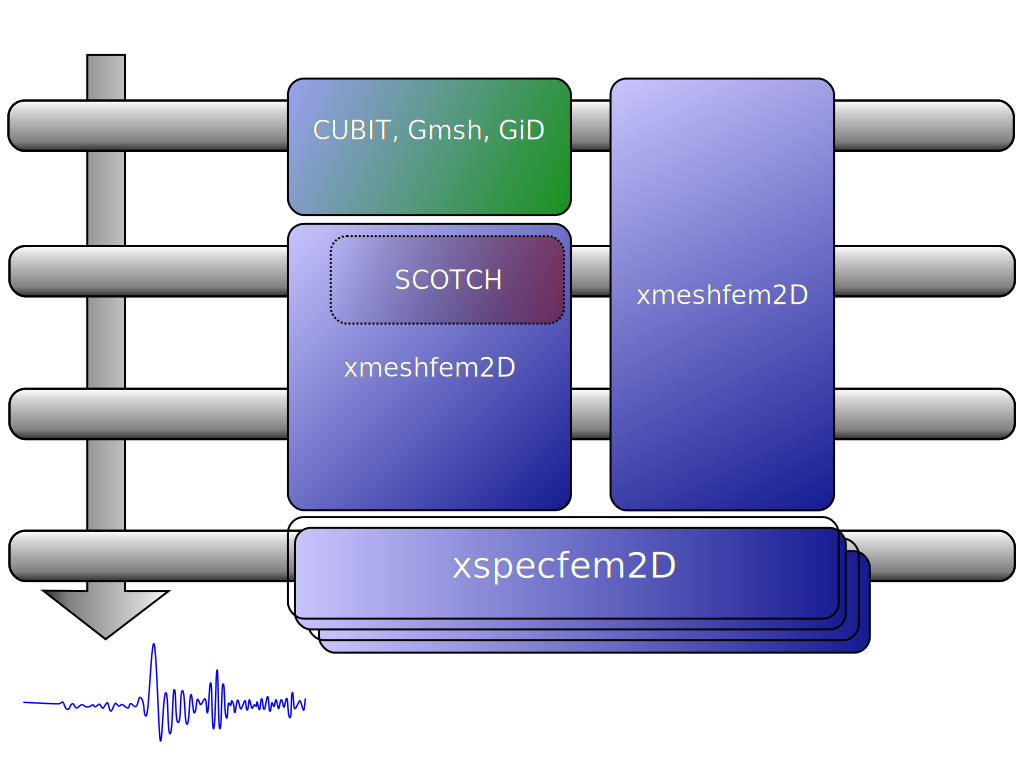
\includegraphics[width=.6\textwidth]{figures/workflow.pdf}

\caption{Schematic workflow for a SPECFEM2D simulation. The executable \texttt{xmeshfem2D} creates the GLL mesh points and assigns specific model parameters. The executable \texttt{xspecfem2D} solves the seismic wave propagation.}

\label{fig:workflow.databases}
\end{figure}

To run the mesher, please follow these steps:
%
\begin{itemize}

\item edit the input file \texttt{DATA/Par\_file}, which describes the simulation.
\red{\textbf{The default \texttt{DATA/Par\_file} provided in the root directory of the code contains detailed comments and should be almost self-explanatory
(note that some of the older \texttt{DATA/Par\_file} files provided in the \texttt{EXAMPLES} directory work fine but some of the comments
they contain may be obsolete or even wrong; thus refer to the default \texttt{DATA/Par\_file} instead for reliable explanations).}}
If you need more details we do not have a detailed description of all the parameters for the 2D version in this manual
but you can find useful information in the manuals of the 3D versions, since many parameters and the general philosophy is similar. They are available at
\urlwithparentheses{https://github.com/geodynamics/specfem3d/tree/master/doc/USER_MANUAL}.
To create acoustic (fluid) regions, just set the S wave speed to zero and the code will see that these elements are fluid and switch to the right equations there automatically, and automatically match them with the solid regions

\item if you are using an external mesher (like GiD or CUBIT / Trelis), you should set \texttt{read\_external\_mesh} to \texttt{.true.}:
  \begin{description}[font=\ttfamily]
     \item[mesh\_file] is the file describing the mesh : first line is the number of elements, then a list of 4 nodes (quadrilaterals only) forming each elements on each line.

     \item[nodes\_coords\_file] is the file containing the coordinates ($x$ and $z$) of each node: number of nodes on the first line, then coordinates x and z on each line.

     \item[materials\_file] is the number of the material for every element : an integer ranging from 1 to \texttt{nbmodels} on each line.

     \item[free\_surface\_file] is the file describing the edges forming the acoustic free surface: number of edges on the first line, then on each line: number of the element, number of nodes forming the free surface (1 for a point, 2 for an edge), the nodes forming the free surface for this element. If you do not want any free surface, just put 0 on the first line; you then get a rigid surface instead.

     \item[axial\_elements\_file] is the file describing the axial elements in the case of an axisymmetric simulation. See Section~\ref{sec:axisym}.
     \item[absorbing\_surface\_file] is the file describing the edges forming the absorbing boundaries:
number of edges on the first line, then on each line: number of the element, number of nodes forming the absorbing edge (must always be equal to 2),
the two nodes forming the absorbing edge for this element, and then the type of absorbing edge: 1 for BOTTOM, 2 for RIGHT, 3 for TOP and 4 for LEFT.
Only two nodes per element can be listed, i.e., the second parameter of each line must always be equal to 2.
If one of your elements has more than one edge along a given absorbing contour
(e.g., if that contour has a corner) then list it twice,
putting the first edge on the first line and the second edge on the second line.
Do not list the same element with the same absorbing edge twice or more, otherwise absorption will not be correct because the edge integral
will be improperly subtracted several times.
If one of your elements has a single point along the absorbing contour rather than a full edge, do NOT list it
(it would have no weight in the contour integral anyway because it would consist of a single point).
If you use 9-node elements, list only the first and last points of the edge and not the intermediate point
located around the middle of the edge; the right 9-node curvature will be restored automatically by the code.

     \item[tangential\_detection\_curve\_file] contains points describing the envelope, that are used for the \texttt{source\_normal\_to\_surface} and \texttt{rec\_normal\_to\_surface}. Should be fine grained, and ordered clockwise. Number of points on the first line, then (x,z) coordinates on each line.
  \end{description}

\item if you have compiled with MPI, you must specify the number of processes.

\end{itemize}
%
Then type
%
\begin{verbatim}
    ./bin/xmeshfem2D
\end{verbatim}
%
to create the mesh (which will be stored in directory \texttt{OUTPUT\_FILES/}). \texttt{xmeshfem2D} is serial; it will output several files called \texttt{Database??????.bin}, one for each process.

%%
\begin{figure}[htbp]
\centering
\includegraphics[width=3in]{figures/example-gridfile.pdf}
\caption{Example of a grid file generated by \texttt{xmeshfem2D} and visualized with gnuplot
(within gnuplot, type `\texttt{plot "OUTPUT\_FILES/gridfile.gnu" w l}').}
\label{fig:example.mesh}
\end{figure}

Regarding mesh point numbering in the files created by the mesher, we use the classical convention of 4-node and 9-node finite elements:
%
\begin{verbatim}
         4 . . . . 7 . . . . 3
         .                   .
         .         eta       .
         .         |         .
         8         9--xi     6
         .                   .
         .                   .
         .                   .
         1 . . . . 5 . . . . 2
\end{verbatim}
%
the local coordinate system being $\xi$ and $\eta$ (\texttt{xi} and \texttt{eta}).
Note that this convention is used to describe the geometry only. In the solver the wave field is then described based on high-order Lagrange interpolants
at Gauss-Lobatto-Legendre points, as is classical in spectral-element methods.

\section{How to use Gmsh to generate an external mesh}

Gmsh%
\footnote{freely available at the following address : \url{http://www.geuz.org/gmsh/}}
is a 3D finite element grid generator which can be used for the generation
of quadrangle and hexahedral meshes. It is therefore a good candidate
for generating meshes which can be processed by SPECFEM2D. Only two
modules of Gmsh are of interest for the SPECFEM2D users : the geometry
and the mesh modules. An example is given in directory \texttt{EXAMPLES/Gmsh\_example}
which illustrates the generation of an external mesh using these two
modules. The model that is considered consists of a homogeneous
square containing two circles filled with a different material.

The geometry is generated by loading file \texttt{SqrCirc.geo} into
Gmsh. The end of the \texttt{.geo} file contains several lines which
are required in order to define the sides of the box and the media.
This is done using the following conventions :
%
\begin{quote}
\texttt{\textit{Physical Line(\textquotedbl Top\textquotedbl)
= \{1\}; }}
\textsf{\textit{\small line corresponding to the top of the box}}

\texttt{\textit{Physical Line(\textquotedbl Left\textquotedbl)
= \{2\}; }}
\textsf{\textit{\small line corresponding to the left side of the box}}

\texttt{\textit{Physical Line(\textquotedbl Bottom\textquotedbl)
= \{3\}; }}
\textsf{\textit{\small line corresponding to the bottom of the box}}

\texttt{\textit{Physical Line(\textquotedbl Right\textquotedbl)
= \{4\}; }}
\textsf{\textit{\small line corresponding to the right side of the box}}

\texttt{\textit{Physical Surface(\textquotedbl M1\textquotedbl)
= \{10\}; }}
\textsf{\textit{\small surrounding medium}}

\texttt{\textit{Physical Surface(\textquotedbl M2\textquotedbl)
= \{11,12\}; }}
\textsf{\textit{\small interior of the two circles}}
\end{quote}
%
For instance, if you want to fill the two circles with two different
materials, you will have to write :
%
\begin{quote}
\texttt{\textit{Physical Surface(\textquotedbl M1\textquotedbl)
= \{10\}; }}
\textsf{\textit{\small surrounding medium}}

\texttt{\textit{Physical Surface(\textquotedbl M2\textquotedbl)
= \{11\}; }}
\textsf{\textit{\small interior of the big circle}}

\texttt{\textit{Physical Surface(\textquotedbl M3\textquotedbl)
= \{12\}; }}
\textsf{\textit{\small interior of the small circle}}
\end{quote}
%
and, consequently, you will have to define a new medium numbered \texttt{3}
in the \texttt{Par\_file}.

\begin{figure}[htbp]
\begin{centering}
\includegraphics[width=0.481\columnwidth]{figures/Gmsh_geo.pdf}
\hspace{2mm}
\includegraphics[width=0.43\columnwidth]{figures/Gmsh_Msh.pdf}
\end{centering}
\caption{Geometry and mesh of the two circle model generated with Gmsh}
\label{fig:Gmsh-example}
\end{figure}

Then, a 2D mesh can be created and saved after selecting the appropriate
options in Gmsh : \texttt{All quads} in \texttt{Subdivision algorithm}
and \texttt{1} or \texttt{2} in \texttt{Element order} whether you
want a 4 or 9 node mesh. This operation will generate a \texttt{SqrCirc.msh}
file which must be processed to get all the files required by SPECFEM2D
when using an external mesh (see previous section). This is done by
running a python script called \texttt{LibGmsh2Specfem.py}, located in
directory \texttt{utils/Gmsh}:
%
\begin{verbatim}
    python LibGmsh2Specfem.py SqrCirc -t A -b A -r A -l A
\end{verbatim}
%
Where the options \texttt{-t}, \texttt{-b},\texttt{ -r} and \texttt{-l}
represent the different sides of the model (top, bottom, right and
left) and can take the values \texttt{A} or \texttt{F} if the corresponding
side is respectively absorbing or free. All boundaries are absorbing
by default. The connections of the generated filenames to the filenames
indicated in the previous section are :
%
\begin{itemize}
\item \texttt{Mesh\_SqrCirc} is the \texttt{\textbf{mesh\_file}}
\item \texttt{Material\_SqrCirc} is the \texttt{\textbf{material\_file}}
\item \texttt{Nodes\_SqrCirc} is the\texttt{ }\texttt{\textbf{nodes\_coords\_file}}
\item \texttt{Surf\_abs\_SqrCirc} is the \texttt{\textbf{absorbing\_surface\_file}}
\item \texttt{Surf\_free\_SqrCirc} is the \texttt{\textbf{free\_surface\_file}}
\end{itemize}
%
In addition, four files like \texttt{free\_surface\_file} corresponding
to the sides of the model are generated.

\section{How to use Cubit/Trelis to generate an external mesh}
Trelis (that was known as Cubit)%
\footnote{available at \url{http://www.csimsoft.com/}}
is a 2D/3D finite element grid generator distributed by Csimsoft which can be
used for the generation of quadrangle and hexahedral meshes. Trelis has a convenient
interface with Python (module cubit) which allows to create meshes from Python scripts. To get
started with Cubit/Trelis we recommend you the step-by-step tutorials available at:
\url{http://www.csimsoft.com/tutorials.jsp}
Many powerful graphical tools are available, and very useful, but we will focus here on
the command line functionalities and especially the Python interface which is the real force of
Cubit/Trelis.

To get started we recommend to the inpatients to open Cubit/Trelis and to click on the
following symbol: \includegraphics[width=0.15in]{figures/play_journal_file.png}. Then select the
files of type Python Files (*.py) and play the following script:
\begin{verbatim}
    utils/cubit2specfem2d/simplest2DexampleWithPmls.py
\end{verbatim}
In the case you want to perform an axisymmetric simulation, we recommend you rather to play:
\begin{verbatim}
    utils/cubit2specfem2d/simpleAxisym2dMesh.py
\end{verbatim}
It will create a simple mesh with PMLs. Then re-click on \includegraphics[width=0.15in]{figures/play_journal_file.png} and
play:
\begin{verbatim}
    utils/cubit2specfem2d/cubit2specfem2d.py
\end{verbatim}
This script will create (in current directory) all the mesh files necessary for a SPECFEM2D simulation.
Other commented examples are available. We particularly recommend you to look at the folder \\ \texttt{EXAMPLES/paper\_axisymmetry\_example}
beginning by reading the README available there.
Read carefully the comments in these scripts, they are helpful.
Another way to use Python together with Cubit/Trelis is to use the script tab.
This tab is a real Python terminal that can be used to pass command line python
instruction to Cubit/Trelis through the cubit module.
In the case of the Script tab is not visible in the command line panel (at the bottom of the screen) do:
\begin{verbatim}
    Tools -> Options... -> Layout [-> Cubit Layout] -> Show script tab
\end{verbatim}
This tab will allow you to play the scripts one line after another directly in Cubit/Trelis.
With this you should be able to understand how to create meshes and export them under SPECFEM2D format.

\subsection{Note about Cubit/Trelis built-in Python}
Beware, there are some (annoying) differences between cubit built-in Python and the actual Python langage:
\begin{itemize}
\item \texttt{"aString" + 'anotherString'} can cause problems even after being stored: \\
      \texttt{a = "aString"} \\
      \texttt{b = a + 'anotherString'} \\
      Example which is not working:
\begin{verbatim}
pathToMeshDir = pathToSpecfem + 'EXAMPLES/paper_axisymmetry_example/MESH'
cubit.cmd('cd \"'+pathToMeshDir+'\"')
\end{verbatim}
\item No comments after double dots: \\
      Example which is not working:
\begin{verbatim}
if True: # Just a dummy comment
    print "Ok!"
\end{verbatim}
      This example works without the comment.
\item \texttt{os.makedirs("\texttildelow/aDirectory/")} does not work. It creates a directory named \texttt{\texttildelow} \\
       !!!!! To remove that do: \texttt{rm -R ./\texttildelow} AND NEVER \texttt{rm -rf \texttildelow} !!!!!
\item \texttt{sys.argv} can not be used
\item No comments \texttt{""" """} at the beginning of a script
\end{itemize}
And probably many others! Think about that before getting mad.

%------------------------------------------------------------------------------------------------%
\section{Notes about absorbing PMLs}
%------------------------------------------------------------------------------------------------%
If you use CPML, an additional file listing the CPML elements is needed.
Its first line is the total number of
CPML elements, and then a list of all the CPML elements, one per line.
The format of these lines is: in the first column the CPML element number, and in the second column a flag as follows:

\begin{table}[hb]
\caption{Definition of flags for CPML elements}
% title of Table
\centering
% used for centering table
\begin{tabular}{c l}
% centered columns (4 columns)
\hline\hline
%inserts double horizontal lines
Flag& Meaning\\ [0.5ex]
% inserts table
%heading
\hline
% inserts single horizontal line
1 & element belongs to a X CPML layer only (either in Xmin or in Xmax)\\
2 & element belongs to a Y CPML layer only (either in Ymin or in Ymax)\\
3 & element belongs to both a X and a Y CPML layer (i.e., to a CPML corner)\\ [1ex]
% [1ex] adds vertical space
\hline
%inserts single line
\end{tabular}
\label{table:CPMLflags}
% is used to refer this table in the text
\end{table}

In order to see how to add PML layers to a mesh / model created with an external mesher such as `Gmsh', see the examples in directory
\texttt{EXAMPLES/CPML\_absorbing\_layers}.

If you use PML, the mesh elements that belong to the PML layers can be acoustic or elastic, but not viscoelastic nor poroelastic.
Then, when defining your model, you should define these absorbing elements as either acoustic or elastic.
If you forget to do that, the code will fix the problem by automatically converting the viscoelastic or poroelastic PML
elements to elastic. This means that strictly speaking the PML layer will not be perfectly matched any more, since the physical
model will change from viscoelastic or poroelastic to elastic at the entrance of the PML, but in practice this is sufficient and
produces only tiny / negligible spurious reflections.

If you use PML and an external mesh (created using an external meshing tool
such as Gmsh, CUBIT/TRELIS or similar), try to have elements inside the PML as regular as possible,
i.e. ideally non-deformed rectangles obtained by `extrusion' of the edge mesh elements meshing the
outer edges of the computational domain without PML; by doing so, the PMLs obtained will be far more stable
in time (PML being weakly unstable from a mathematical point of view, very deformed mesh elements
inside the PMLs can trigger instabilities much more quickly).

If you have an existing CUBIT (or similar) mesh stored in SPECFEM2D
format but do not know how to assign CPML flags to it,
we have created a small serial Fortran program that will do that automatically for you.
That program is utils/CPML/convert\_external\_layers\_of\_a\_given\_mesh\_to\_CPML\_layers2D.f90.
When you create the PML layers using that script, you do not need to mark
(i.e. assign to physical entities with a specific name) those external layers in the mesher.
However you still need to specify the boundary of the mesh as you where doing in the case of absorbing conditions.
The script will automatically extract the elements on the PML. It will ask you for a thickness for the PML layers.
Suppose that you have created a region with a 1-meter size element, when it will prompt for the PML thickness
you can enter 3.1 and it will create a PML 3 element thick. Always input a slightly larger (5-10\%) size because the element might be slightly skewed,
or if you have not created your PML region via extrusion/webcut in CUBIT/TRELIS.

To stabilize PMLs it also helps to add a transition layer of geometrically-regular non-PML elements, in which attenuation is also
turned off (i.e. $Q_\kappa = Q_\mu = 9999$ in that layer), as in the red layer of Figure~\ref{fig:mesh_extrusion}.
Our tools in directory in directory utils/CPML \red{should soon (Dimitri: TO DO ONE DAY)} implement that transition layer automatically.

To be more precise:

1/ If one wants to use PML layers, they should NOT mark the layers according to that python script - the reason is that the xmeshfem2d does not recognize those CPML flags. If whoever developed the script adjusts it to solve this problem - this might be a great relief for users; as of now no physical identifiers are needed for those layers.

2/ HOWEVER, the "Top", "Bottom", "Left"," and "Right" boundaries of the model, need to be re-assigned to outer boundaries of the model - that will be the leftmost boundary of the left -bounding PML , rightmost of the right PML, topmost for the Top PML (if there is one) and the bottom boundary of the bottom layer. Those and only those lines need to have the mentioned identifiers (opposite to the example with the two-holed square with Stacey conditions).

3/ There is no need to create Top PML in case one wants it to be reflective; as the fortran script that assigns the flag will ignore the elements that sit within  PML-layer thickness distance to the top.

4/ The Fortran program utils/CPML/convert\_external\_layers\_of\_a\_given\_mesh\_to\_CPML\_layers2D.f90
that flags the PML elements does not create additional elements; it simply takes the elements within chosen distance from the boundaries, that sit in the interior of model and marks them as absorbing.

If you use PML and an external velocity and density model (e.g., setting flag ``\texttt{MODEL}'' to \texttt{tomography}),
you should be careful because mathematically a PML cannot handle heterogeneities along the
normal to the PML edge inside the PML layer. This comes from the fact that the damping profile
that is defined assumes a constant velocity and density model along the normal
direction.
Thus, you need to modify your velocity and density model in order for it to be 1D inside
the PML, as shown in Figure~\ref{fig:modify_external_velocity_model_to_use_PML}.
This applies to the bottom layer as well; there you should make sure
that your model is 1D and thus constant along the vertical direction.
To summarize, only use a 2D velocity and density model inside the physical region, and in
all the PML layers extend it by continuity from its values along the
inner PML edge.

%%
\begin{figure}[htbp]
\noindent \begin{centering}
\includegraphics[width=4.5in]{figures/how_to_use_a_transition_mesh_layer_to_stabilize_PML.png}
\par\end{centering}
\caption{Mesh extrusion for PML (green elements) and a non-PML stabilization layer (red elements).}
\label{fig:mesh_extrusion}
\end{figure}
%%

%%
\begin{figure}[htbp]
\centering
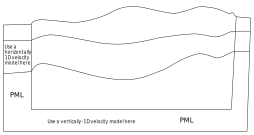
\includegraphics[width=6in]{figures/how_to_use_PML_with_external_velocity_model.pdf}
\caption{How to modify your external 2D velocity and density model in order to use PML.
Such a modification is not needed when using Stacey absorbing boundary conditions (but such conditions
are significantly less efficient).}
\label{fig:modify_external_velocity_model_to_use_PML}
\end{figure}
%%

%------------------------------------------------------------------------------------------------%
\section{Controlling the quality of an external mesh}
%------------------------------------------------------------------------------------------------%

To examine the quality of the elements in your externally build mesh, type
%
\begin{verbatim}
    ./bin/xcheck_quality_external_mesh
\end{verbatim}
%
(and answer "3" to the first question asked).
This code will tell you which element in the whole mesh has the worst quality (maximum skewness, i.e. maximum deformation of the element angles) and it should be enough to modify this element with the external software package used for the meshing, and
to repeat the operation until the maximum skewness of the whole mesh is less or equal to about 0.75 (above is dangerous: from 0.75 to 0.80 could still work, but if there is a single element above 0.80 the mesh should be improved).

The code also shows a histogram of 20 classes of skewness which tells how many element are above the skewness = 0.75, and to which percentage of the total this amounts. To see this histogram, you could type:
%
\begin{verbatim}
    gnuplot plot_mesh_quality_histogram.gnu
\end{verbatim}
%
This tool is useful to estimate the mesh quality and to see it evolve along the successive corrections.

%------------------------------------------------------------------------------------------------%
\section{Controlling how the mesh samples the wave field}
%------------------------------------------------------------------------------------------------%

To examine (using Gnuplot) how the mesh samples the wave field, type
%
\begin{verbatim}
    gnuplot plot_points_per_wavelength_histogram.gnu
\end{verbatim}
%
and also check the following histogram printed on the screen or in the output file:
%
\begin{verbatim}
    histogram of min number of points per S wavelength (P wavelength in
    acoustic regions)
    (too small: poor resolution of calculations - too big = wasting
    memory and CPU time)
    (threshold value is around 4.5 points per wavelength in elastic media
    and 5.5 in acoustic media)
\end{verbatim}

If you see that you have a significant number of mesh elements below the threshold indicated, then your simulations
will not be accurate and you should create a denser mesh. Conversely, if you have a significant number of mesh elements above the threshold indicated,
the mesh your created is too dense, it will be extremely accurate but the simulations will be slow; using a coarser mesh would be sufficient and would lead to faster simulations.




%------------------------------------------------------------------------------------------------%

\chapter{Running the Solver xspecfem2D}

%------------------------------------------------------------------------------------------------%

To run the solver, type
%
\begin{verbatim}
    bin/xspecfem2D
\end{verbatim}
%
from within the main working directory (use \texttt{mpirun} or equivalent if you compiled with parallel support). This will output the seismograms and snapshots of the wave fronts at different time steps in directory \texttt{OUTPUT\_FILES/}. To visualize them, type "\texttt{gs OUTPUT\_FILES/vect*.ps}" to see the Postscript files (in which the wave field is represented with small arrows, fluid/solid matching interfaces with a thick pink line, and absorbing edges with a thick green line) and "\texttt{gimp OUTPUT\_FILES/image*.gif}" to see the colour snapshot showing a pixelized image of one of the two components of the wave field (or pressure, depending on what you have selected for the output in \texttt{DATA/Par\_file}).

%%
\begin{figure}[htbp]
\centering
\includegraphics[width=2in]{figures/image0000300.jpg}
\includegraphics[width=2in]{figures/image0000400.jpg}
\includegraphics[width=2in]{figures/image0000500.jpg}
\caption{Wavefield snapshots of the default example generated by \texttt{xspecfem2D} when parameter \texttt{output\_color\_image} is set to \texttt{.true.}. To create smaller (subsampled) images you can change double precision parameter \texttt{factor\_subsample\_image = 1.0} to a higher value in file \texttt{DATA/Par\_file}. This can be useful in the case of very large models. The number of pixels of the image in each direction must be smaller than parameter \texttt{NX\_NZ\_IMAGE\_MAX} defined in file \texttt{SETUP/constants.h.in}, again to avoid creating huge images in the case of very large models.}
\label{fig:example.solver}
\end{figure}
%%

Please consider these following points, when running the solver:
%
\begin{itemize}
\item the \texttt{DATA/Par\_file} given with the code works fine, you can use it without any modification to test the code

\item the seismograms \texttt{OUTPUT\_FILES/*.sem*} are simple ASCII files with two columns: time in the first column and amplitude in the second, therefore they can be visualized with any tool you like, for instance ``\texttt{gnuplot}''; if you prefer to output binary seismograms in Seismic Unix format (which is a simple binary array dump) you can use parameter \texttt{SU\_FORMAT}, in which case all the seismograms will be written to a single file with the extension \texttt{*.bin}.
Depending on your installation of the Seismic Unix package you can use one of these two commands:
%
\begin{verbatim}
    surange < Uz_file_single.bin
    suoldtonew < Uz_file_single.bin | surange
\end{verbatim}
%
to see the header info.
Replace \texttt{surange} with \texttt{suxwigb} to see wiggle plots for the seismograms.

\item if flag \texttt{MODEL} in \texttt{DATA/Par\_file} is set to \texttt{default}, the velocity and density model is determined using the \texttt{nbmodels} and \texttt{nbregions} devices.  Otherwise, \texttt{nbmodels} values are ignored and the velocity and density model is determined from a user supplied file or subroutine.

\item when compiling with Intel ifort, use ``\texttt{-assume byterecl}'' option to create binary PNM images displaying the wave field

\item there are a few useful scripts and Fortran routines in directory \texttt{utils/}.

\item you can find a Fortran code to compute the analytical solution for simple media that we use as a reference in benchmarks in many of our articles at
\urlwithparentheses{http://www.spice-rtn.org/library/software/EX2DDIR}. That code is described in: \cite{BeIfNiSk94}

\end{itemize}

%------------------------------------------------------------------------------------------------%
\section*{Notes about \texttt{DATA/Par\_file} parameters}
%------------------------------------------------------------------------------------------------%

\red{\textbf{The default \texttt{DATA/Par\_file} provided in the root directory of the code contains detailed comments and should be almost self-explanatory
(note that some of the older \texttt{DATA/Par\_file} files provided in the \texttt{EXAMPLES} directory work fine but some of the comments
they contain may be obsolete or even wrong; thus refer to the default \texttt{DATA/Par\_file} instead for reliable explanations).}}

\begin{description}[font=\ttfamily]

\item[USE\_TRICK\_FOR\_BETTER\_PRESSURE]

This option can only be used so far if all the receivers record pressure and are in acoustic elements.
Use a trick to increase accuracy of pressure seismograms in fluid (acoustic) elements:
use the second derivative of the source for the source time function instead of the source itself,
and then record \texttt{potential\_acoustic()} as pressure seismograms instead of \texttt{potential\_dot\_dot\_acoustic()};
this is mathematically equivalent, but numerically significantly more accurate because in the explicit
Newmark time scheme acceleration is accurate at zeroth order while displacement is accurate at second order,
thus in fluid elements \texttt{potential\_dot\_dot\_acoustic()} is accurate at zeroth order while \texttt{potential\_acoustic()}
is accurate at second order and thus contains significantly less numerical noise.

%use a trick to increase accuracy of pressure seismograms in fluid (acoustic) elements: use the second derivative of the source for the source time function instead of the source itself, and then record -potential\_acoustic() as pressure seismograms instead of -potential\_dot\_dot_acoustic(); this is mathematically equivalent, but numerically significantly more accurate because in the explicit Newmark time scheme acceleration is accurate at zeroth order while displacement is accurate at second order, thus in fluid elements potential\_dot\_dot_acoustic() is accurate at zeroth order while potential\_acoustic() is accurate at second order and thus contains significantly less numerical noise.


\item[READ\_VELOCITIES\_AT\_f0]

 shift (i.e. change) velocities read from the input file to take average physical dispersion into account, i.e. if needed change the reference frequency at which these velocities are defined internally in the code: by default, the velocity values that are read at the end of this Par\_file of the code are supposed to be the unrelaxed values, i.e. the velocities at infinite frequency. If you set this flage to .true., the values read are then those for a given frequency called ATTENUATION\_f0\_REFERENCE.


\item[nbmodels]  With \texttt{MODEL = default} chosen, a variety of simple velocity and density models can be defined using the \texttt{nbmodels} device.

%
\begin{verbatim}
I:  model_number 1 rho Vp Vs 0 0 QKappa Qmu 0 0 0 0 0 0
II:  model_number 2 rho c11 c13 c15 c33 c35 c55 c12 c23 c25 0 0 0
III: model_number 3 rhos rhof phi c kxx kxz kzz Ks Kf Kfr etaf mufr Qmu
IV: model_number -1 0 0 A 0 0 0 0 0 0 0 0 0 0
\end{verbatim}
%

To make a given region acoustic, use I and make \texttt{Vs} be zero.

To make a given region isotropic elastic, use I and make \texttt{Vs} be nonzero.  See Section 4.1 for more details.

To make a given region anisotropic, use II.  See Section 4.2 for more details.

To make a given region poroeslatic, use III.  See Section 4.3 for more details.

When viscoelasticity is turned on, the \texttt{Vp} and \texttt{Vs} values that are read here are the UNRELAXED ones i.e. the values at infinite frequency
unless the READ\_VELOCITIES\_AT\_f0 parameter above is set to true, in which case they are the values at frequency $f_0$.
Please also note that Qmu is always equal to Qs, but Qkappa is in general not equal to Qp. To convert one to the other see doc/note\_on\_Qkappa\_versus\_Qp.pdf and utils/attenuation/conversion\_from\_Qkappa\_Qmu\_to\_Qp\_Qs\_from\_Dahlen\_Tromp\_959\_960.f90.

\item[nbregions]  With \texttt{MODEL = default} chosen, a variety of simple layered model configurations can be specified using the \texttt{nbregions} device.



\end{description}

Regarding attenuation (viscoelasticity), in the Par\_file you need to select the number of standard linear solids (N\_SLS) to use to mimic a constant $Q$ quality factor.
Using N\_SLS = 3 is always safe. If (and only if) you know what you are doing, you can try to reduce that in order to reduce the cost of the simulations.
Figure~\ref{fig:selectNSLS} shows values that you can consider using (again, if and only if you know what you are doing). That table has been created by Zhinan Xie using
a comparison between results obtained with a truly-constant $Q$ and results obtained with its approximation based on N\_SLS standard linear solids.
The comparison is performed using the time-frequency misfit and goodness-of-fit criteria proposed by \cite{Kristekova_2009}.
The table is drawn for a dimensionless parameter representing the distance of propagation.
%%
\begin{figure}[htbp]
\centering
\includegraphics[width=5in]{figures/minimum_number_of_SLS_that_can_be_used_in_viscoelastic_simulation.png}
\caption{Table showing how you can select a value of N\_SLS smaller than 3, if and only if you know what you are doing.}
\label{fig:selectNSLS}
\end{figure}
%%


%------------------------------------------------------------------------------------------------%
\section*{Notes about \texttt{DATA/SOURCE} parameters}
%------------------------------------------------------------------------------------------------%


The \texttt{SOURCE} file located in the \texttt{DATA/} directory should be edited in the following way:
%
\begin{description}[font=\ttfamily]
\item[source\_surf] Set this flag to \texttt{.true.} to force the source to be located at the surface of the model, otherwise
the sol be placed inside the medium

\item[xs] source location $x$ in meters

\item[zs] source location $z$ in meters

\item[source\_type] Set this value equal to \texttt{1} for elastic forces or acoustic pressure,
set this to \texttt{2} for moment tensor sources.
For a plane wave including converted and reflected waves at the free surface, P wave = 1, S wave = 2, Rayleigh wave = 3;
for a plane wave without converted nor reflected waves at the free surface, i.e. the incident wave only, P wave = 4, S wave = 5.
(incident plane waves are turned on by parameter \texttt{initialfield} in \texttt{DATA/Par\_file}).

\item[time\_function\_type] Choose a source-time function: set this value to \texttt{1} to use a Ricker, i.e. the second derivative of a Gaussian,
\texttt{2} to use the first derivative of a Gaussian, \texttt{3} to use a Gaussian, \texttt{4} to use a Dirac or \texttt{5} to use a Heaviside source-time function.
Note that we use the standard definition of a Ricker, for a dominant frequency $f_0$:
$\mathrm{Ricker}(t) = (1 - 2 a t^2) e^{-a t^2}$, with $a = \pi^2 f_0^2$,
whose Fourier transform is thus:
$\frac{1}{2} \frac{\sqrt{\pi}\omega^2}{a^{3/2}}e^{-\frac{\omega^2}{4 a}}$
This gives the wavelet of Figure~\ref{fig:RickerWavelet}.
%%
\begin{figure}[htbp]
\centering
\includegraphics[width=3in]{figures/Ricker_wavelet.png}
\caption{We use the standard definition of a Ricker (i.e., second derivative of a Gaussian). Image taken from \url{http://subsurfwiki.org}.}
\label{fig:RickerWavelet}
\end{figure}
%%

\item[f0] Set this to the dominant frequency of the source.
For point-source simulations using a Heaviside source-time function (\texttt{time\_function\_type = 5}),
we recommend setting the source frequency parameter \texttt{f0}
equal to a high value, which corresponds to simulating a step source-time
function, i.e., a moment-rate function that is a delta function.

The \texttt{half duration} of a source is obtained by $1/\mathtt{f0}$.
If the code will use a Gaussian source-time function (\texttt{time\_function\_type = 3})
(i.e., a signal with a shape similar to a `smoothed triangle', as
explained in \citet{KoTr02a} and shown in Fig~\ref{fig:gauss.vs.triangle}), the
source-time function uses a half-width of \texttt{half duration}. We prefer
to run the solver with \texttt{half duration} set to zero and convolve
the resulting synthetic seismograms in post-processing after the run,
because this way it is easy to use a variety of source-time functions.
\citet{KoTr02a} determined
that the noise generated in the simulation by using a step source
time function may be safely filtered out afterward based upon a convolution
with the desired source time function and/or low-pass filtering. Use
the serial code \texttt{convolve\_source\_timefunction.f90} and the
script \texttt{convolve\_source\_timefunction.sh} for this purpose,
or alternatively use signal-processing software packages such as SAC \urlwithparentheses{www.llnl.gov/sac}.
Type
%
\begin{verbatim}
    make xconvolve_source_timefunction
\end{verbatim}
%
to compile the code and then set the parameter \texttt{hdur} in \texttt{convolve\_source\_timefunction.sh}
to the desired half-duration.
%%
\begin{figure}[htbp]
\centering
\includegraphics[width=3in]{figures/gauss_vs_triangle_mod.pdf}
\caption{Comparison of the shape of a triangle and the Gaussian function actually
used.}
\label{fig:gauss.vs.triangle}
\end{figure}
%%

\item[t0] For single sources, we recommend to set the time shift parameter \texttt{t0} equal to $0.0$.
The time shift parameter would simply apply
an overall time shift to the synthetics (according to the time shift of the first source), something that can be done
in the post-processing. This time shift parameter can be non-zero when using multiple sources.

\item[anglesource] angle of the source (for a force only); for a plane wave, this is the incidence angle. For moment tensor sources this parameter is unused.

\item[Mxx,Mzz,Mxz] Moment tensor components (valid only for moment tensor sources, \texttt{source\_type = 2}).
Note that the units for the components of a moment tensor source are different in SPECFEM2D and in SPECFEM3D:
%
\begin{description}
\item[SPECFEM3D:] in SPECFEM3D the moment tensor components are in dyne*cm
\item[SPECFEM2D:] in SPECFEM2D the moment tensor components are in N*m
\end{description}

To go from strike / dip / slip to CMTSOLUTION moment-tensor format using the classical formulas (of e.g. \cite{AkRi80} you can use these two small C programs from \texttt{SPECFEM3D\_GLOBE}:

\texttt{./utils/strike\_dip\_rake\_to\_CMTSOLUTION.c}

\texttt{./utils/CMTSOLUTION\_to\_AkiRichards.c}

but then it is another story to make a good 2D approximation of that, because in plain-strain P-SV what you get is the equivalent of a line source in the third direction (orthogonal to the plane) rather than a 3D point source
For more details on this see e.g. Section 7.3 "Two-dimensional point sources" of the book of \cite{Pil79}. That book being hard to find, we scanned the related pages in file\\
\texttt{discussion\_of\_2D\_sources\_and\_approximations\_from\_Pilant\_1979.pdf} in the same directory as this users manual.
Another very useful reference addressing that is \cite{HeVi88} and its recent extension \citep{LiHeClSu14}.

\item[factor] amplification factor

\end{description}

Note, the zero time of the simulation corresponds to the center of the triangle/Gaussian,
or the centroid time of the earthquake. The start time of the simulation
is $t=-1.2*\mathtt{half~duration} + \mathtt{t0}$ (the factor 1.2 is to make sure the moment
rate function is very close to zero when starting the simulation; Heaviside functions use a factor 2.0),
the half duration is obtained by $1/\mathtt{f0}$.
If you prefer, you can fix this start time by setting the parameter \texttt{USER\_T0} in the \texttt{constants.h} file
to a positive, non-zero value. The simulation in that case would start at a starting time equal to \texttt{-USER\_T0}.


%------------------------------------------------------------------------------------------------%
\section{How to run elastic wave simulations}
%------------------------------------------------------------------------------------------------%

For isotropic elastic materials, there are two options:
%
\begin{description}
\item[P-SV:]
To run a P-SV waves calculation propagating in the $x$-$z$ plane,
set \texttt{p\_sv = .true.} in the \texttt{Par\_file}.

\item[SH:]
To run a SH (membrane) waves calculation travelling in the $x$-$z$ plane with a
$y$-component of motion, set \texttt{p\_sv = .false.}

\end{description}
%
This feature is only implemented for elastic materials and sensitivity kernels
can be calculated (see \cite{TaLiTr07} for details on membrane
surface waves).

An optional useful Python script called \texttt{SEM\_save\_dir.py} is provided.
It allows one to automatically save all the parameters and results of a given simulation.
%------------------------------------------------------------------------------------------------%

%------------------------------------------------------------------------------------------------%
\section{How to run axisymmetric wave simulations}
\label{sec:axisym}
%------------------------------------------------------------------------------------------------%
Axisymmetric simulations are possible in SPECFEM2D. For these simulations the 2D domain simulated is physically the meridional 2D shape of an axisymmetric 3D domain.
We invite you to read our publication \citep{BoCrKoAs16} as an introduction.
To set the geometry as axisymmetric turn the flag \texttt{AXISYM} to \texttt{.true.} in the \texttt{Par\_file}:
\begin{verbatim}
   AXISYM                          = .true.
\end{verbatim}
The left border of the model becomes then a symmetry axis. The wavefield calculated is then physically a 3D wavefield obtained by revolution of a 2D wavefield
around its left border.
\\\\
Note about the source:\\
In axisymmetric geometry the whole model is symmetric with respect to this axis, including the source. Hence if the source is not on the axis it will physically
have a circular shape. This is still possible and relevant for some applications as non destructive testing but
is most of the time unwanted. This has to be kept in mind. In acoustic medium, as an explosion in a fluid is naturally axisymmetric, the wavefield generated has the
correct 3D shape. However, if the source is put in an elastic solid, its 3D radiation pattern will be axisymmetric.
\\\\
Getting started:\\
To get started a simple example is available in
\texttt{EXAMPLES/axisymmetric\_case\_AXISYM\_option}, we encourage you to read the \texttt{README} file you will find there.
This example contains an example of the use of \texttt{AXISYM} option plus a validation using the semi-analytical code OASES (\cite{Oases2004}).
In this example the domain studied is a water layer lying above a viscoelastic medium. The source is an explosion in the water and the domain is bounded with PMLs.
\\\\
Note about external meshers:\\
Using external meshers is possible in axisymmetric geometry. An example is available in \\ \texttt{EXAMPLES/paper\_axisymmetry\_example} with the mesher
Cubit/Trelis (\url{http://www.csimsoft.com/trelis}).
We invite you to check this example and read the previous chapter for more details. The only difference with plane-strain geometry is that SPECFEM2D needs an additional file defining
axial elements. The path to this file has to be given in the \texttt{Par\_file}:
\begin{verbatim}
   axial_elements_file             = /path/to/the/axial_elements_file
\end{verbatim}
The axial elements file has the following structure:
\begin{verbatim}
        48
         1          2       8456       8457
         2          2       8457       8458
         3          2       8458       8459
         4          2       8459       8460
       623          2        171        204
      1053          2        172       9512
      1054          2        172        173
      1055          2        173        174
      ...
\end{verbatim}
Which is similar to free surface files. Hence the first line contains the number of axial elements, then the other lines contain four columns:
element id, number of nodes describing an axial element (always 2), first node id, second node id.
Note that the axis elements must include the possible (up and/or down) PMLs elements in contact with the axis.
For simplicity we assume that the mesh elements that are in contact with the symmetry axis are in contact with it
by a full edge rather than by a single point, i.e. we exclude cases as that of Figure~\ref{fig:meshrestrictionontheaxis}.
This amounts to imposing that the leftmost layer of elements in the mesh be structured rather than non structured; The rest of the mesh can be non structured.
\begin{figure}
%\centerline{\includegraphics[width=0.38\linewidth]{FIGURES/case_that_we_exclude_for_axisymmetric_mesh.eps}}
\centerline{\includegraphics[width=0.38\linewidth]{figures/meshrestrictionontheaxis-eps-converted-to.pdf}}
\caption{\label{fig:meshrestrictionontheaxis} For simplicity we exclude cases in which the mesh elements that are in contact with the symmetry axis
are in contact with it by a single point instead of by a full edge, such as element $\bar{\Omega}_2$ here.
This amounts to imposing that the leftmost layer of elements in the mesh be structured rather than non structured; The rest of the mesh can be non structured.}
\end{figure}
\\\\
Note about the resolution:\\
In axisymmetry a different quadrature is used in the axial elements making the number of points per wavelength necessary a slightly
bigger ($\approx 25\%$) than in plane-strain.
\\\\
Note about a small remaining bug:\\
It has to be noted that a small bug is still hiding somewhere in the code. Indeed the output signals generated are correct in the
whole domain except in the element containing the source. This small bug has not been solved so far but not prevent to use the code.
\\\\
Note about a demo code to learn:\\
A simplistic demo code is available in \\ \texttt{utils/small\_SEM\_solver\_in\_Fortran\_without\_MPI\_to\_learn}.
This simple code is useful to learn how the spectral-element method works in both plane-strain and axisymmetric geometries.
Have a look to it if interested. Once in its directory, type \texttt{./make\_Fortran\_2D\_axisymmetric.csh} and then \texttt{./xspecfem2D}
to compile and run. The bug discussed above is not present in this small code.
%------------------------------------------------------------------------------------------------%

%------------------------------------------------------------------------------------------------%
\section{How to run anisotropic wave simulations}
%------------------------------------------------------------------------------------------------%

Following \cite{CaKoKo88}, we use the classical reduced Voigt notation to represent symmetric
tensors \citep{Hel94,Car07}:
%
\begin{quotation}
The constitutive relation of a heterogeneous anisotropic and elastic solid
is expressed by the generalized Hooke's law, which can be written as
%
\begin{equation*}
\sigma_{ij} = c_{ijkl} \varepsilon_{kl}, \qquad i, j, k = 1, \dots, 3,
\end{equation*}
%
where $t$ is the time, $\mathbf{x}$ is the position vector, $\sigma_{ij}(\mathbf{x}, t)$ and $\varepsilon_{ij}(\mathbf{x}, t)$ are the
Cartesian components of the stress and strain tensors respectively, and
$c_{ijkl}(\mathbf{x})$ are the components of a fourth-order tensor called the elasticites of
the medium. The Einstein convention for repeated indices is used.

To express the stress-strain relation for a transversely isotropic medium
we introduce a shortened matrix notation commonly used in the literature.
With this convention, pairs of subscripts concerning the elasticities are
replaced by a single number according to the following correspondence:
%
\begin{align*}
(11) \rightarrow 1, &&
(22) \rightarrow 2, &&
(33) \rightarrow 3, \\
(23) = (32) \rightarrow 4, &&
(31) = (13) \rightarrow 5, &&
(12) = (21) \rightarrow 6.
\end{align*}
\end{quotation}
%
Thus in the most general 2D case we have the following convention for the stress-strain relationship:
%
\begin{verbatim}
! implement anisotropy in 2D
sigma_xx = c11*dux_dx + c13*duz_dz + c15*(duz_dx + dux_dz)
sigma_zz = c13*dux_dx + c33*duz_dz + c35*(duz_dx + dux_dz)
sigma_xz = c15*dux_dx + c35*duz_dz + c55*(duz_dx + dux_dz)

! sigma_yy is not equal to zero in the plane strain formulation
! but is used only in post-processing if needed,
! to compute pressure for display or seismogram recording purposes
sigma_yy = c12*dux_dx + c23*duz_dz + c25*(duz_dx + dux_dz)
\end{verbatim}
%
where the notations are for instance \texttt{duz\_dx = d(Uz) / dx}.


%------------------------------------------------------------------------------------------------%
\section{How to run poroelastic wave simulations}
%------------------------------------------------------------------------------------------------%

Check the following new inputs in \texttt{Par\_file}:
%
\begin{description}[style=nextline, labelindent=1em, font=\normalfont]
\item[In section \textbf{"\# geometry of model and mesh description"}:]
\texttt{TURN\_VISCATTENUATION\_ON}, \texttt{Q0}, and \texttt{FREQ0} deal with viscous damping in a poroelastic medium.
\texttt{Q0} is the quality factor set at the central frequency \texttt{FREQ0}. For more details
see \cite{MoTr08}.

\item[In section \textbf{"\# time step parameters"}:]
\texttt{SIMULATION\_TYPE} defines the type of simulation
  \begin{enumerate}[label=(\arabic*)]
    \item forward simulation
    \item UNUSED (purposely, for compatibility with the numbering convention used in our 3D codes)
    \item adjoint method and kernels calculation
  \end{enumerate}

\item[In section \textbf{"\# source parameters"}:]
The code now support multiple sources.
\texttt{NSOURCE} is the number of sources.
Parameters of the sources are displayed in the file \texttt{SOURCE}, which must be
in the directory \texttt{DATA/}. The components of a moment tensor source must be given in N.m,
not in dyne.cm as in the \texttt{DATA/CMTSOLUTION} source file of the 3D version of the code.
%%%
\begin{figure}[htbp]
\centering
\includegraphics[width=5in]{figures/source_timing.pdf}
\caption{Example of timing for three sources. The center of the first source
triangle is defined to be time zero. Note that this is NOT in general
the hypocentral time, or the start time of the source (marked as \texttt{tstart}).
The time shift parameter \texttt{t0} in the \texttt{SOURCE} file
would be $t1(=0)$, $t2$, $t3$ in this case, and the half-duration parameter, \texttt{f0},
would be $\mathtt{hdur1}=1/\mathtt{f0}_1$, $\mathtt{hdur2}=1/\mathtt{f0}_2$,
$\mathtt{hdur3}=1/\mathtt{f0}_3$ for the sources 1, 2, 3 respectively.}
\label{fig:source_timing}
\end{figure}
%%%


\item[In section \textbf{"\# receiver line parameters for seismograms"}:]
\texttt{SAVE\_FORWARD} determines if the last frame of a forward simulation is saved (\texttt{.true.}) or not (\texttt{.false})

\item[In section \textbf{"\# define models...."}:]
There are three possible types of models:
  \begin{enumerate}[label=\ttfamily \Roman*:]
    \item (\texttt{model\_number 1 rho Vp Vs 0 0 QKappa Qmu 0 0 0 0 0 0}) or
    \item (\texttt{model\_number 2 rho c11 c13 c15 c33 c35 c55 c12 c23 c25 0 0 0}) or
    \item (\texttt{model\_number 3 rhos rhof phi c kxx kxz kzz Ks Kf Kfr etaf mufr Qmu}).
  \end{enumerate}

For isotropic elastic/acoustic material use \texttt{I} and set \texttt{Vs} to zero to make a given model acoustic, for anisotropic elastic use \texttt{II},
and for isotropic poroelastic material use \texttt{III}. The mesh can contain acoustic, elastic, and poroelastic models simultaneously.

For anisotropic elastic media the last three parameters, \texttt{c12 c23 c25}, are used only when the user asks the code to compute pressure for display
or seismogram recording purposes. Thus, if you do not know these parameters for your anisotropic material and/or if you do not plan to display or record pressure you
can ignore them and set them to zero. When pressure is used these three parameters are needed because the code needs to compute $\sigma_{yy}$,
which is not equal to zero in the plane strain formulation.

\begin{description}[font=\ttfamily, labelindent=1em, labelsep=1ex]
\item[rho\_s] = solid density
\item[rho\_f] = fluid density
\item[phi] = porosity
\item[tort] = tortuosity
\item[permxx] = xx component of permeability tensor
\item[permxz] = xz,zx components of permeability tensor
\item[permzz] = zz component of permeability tensor
\item[kappa\_s] = solid bulk modulus
\item[kappa\_f] = fluid bulk modulus
\item[kappa\_fr] = frame bulk modulus
\item[eta\_f] = fluid viscosity
\item[mu\_fr] = frame shear modulus
\item[Qmu] = shear quality factor
\end{description}

Note: for the poroelastic case, \texttt{mu\_s} is irrelevant.
For details on the poroelastic theory see \cite{MoTr08}.

\end{description}

\texttt{get\_poroelastic\_velocities.f90} allows to compute cpI, cpII, and cs function of
the source dominant frequency. Notice that for this calculation we use \texttt{permxx}
and the dominant frequency of the first source, f0(1). Caution if you use
several sources with different frequencies and if you consider anistropic
permeability.

%------------------------------------------------------------------------------------------------%
\section{Coupled simulations}
%------------------------------------------------------------------------------------------------%

The code supports acoustic/elastic, acoustic/poroelastic, elastic/poroelastic,
and acoustic, elastic/poroelastic simulations.
Elastic/poroelastic coupling supports anisotropy, but not attenuation for the
elastic material.


%------------------------------------------------------------------------------------------------%
\section{How to choose the time step}
%------------------------------------------------------------------------------------------------%

Three different explicit conditionally-stable time schemes can be used for elastic, acoustic (fluid) or coupled elastic/acoustic media:
the Newmark method, the low-dissipation and low-dispersion fourth-order six-stage Runge-Kutta method (LDDRK4-6) presented in \cite{BeBoBa06},
and the classical fourth-order four-stage Runge-Kutta (RK4) method.
Currently the last two methods are not implemented for poroelastic media.
According to \cite{DeSe10} and \cite{BeBoBa06}, with different degrees $N=NGLLX-1$ of the GLL basis functions the CFL bounds are given in the following tables.
Note that by default the SPECFEM solver uses $NGLLX = 5$ and thus a degree $N = 4$, which is thus the value you should use
in most cases in the following tables.
You can directly compare these values with the value given in sentence `Max stability for P wave velocity' in file
\texttt{output\_solver.txt} to see whether you set the correct $\Delta t$ in \texttt{Par\_file} or not.
For elastic simulation, the
CFL value given in \texttt{output\_solver.txt} does not consider the $V_p/V_s$ ratio, but the CFL limit slight decreases when $V_p/V_s$ increases.
In viscoelastic simulations the CFL limit does not change compared to the elastic case because we use a rational approximation of a constant quality factor Q, which has no attenuation effect on zero-frequency waves.
Additionally, if you use C-PML absorbing layers in your simulations, which are implemented for the Newmark and LDDRK4-6 techniques but not for the classical RK4), the CFL upper limit decreases to approximately 95\% of the limit without absorbing layers in the case of Newmark and to 85\% in the case of LDDRK4-6.
\begin{table}[htbp]
\caption{CFL upper bound for an acoustic (fluid) simulation.}
% title of Table
\centering
% used for centering table
\begin{tabular}{c c c c}
% centered columns (4 columns)
\hline\hline
%inserts double horizontal lines
Degree $N$ & Newmark & LDDRK4-6 & RK4 \\ [0.5ex]
% inserts table
%heading
\hline
% inserts single horizontal line
1 & 0.709 & 1.349 & 1.003 \\
2 & 0.577 & 1.098 & 0.816 \\
3 & 0.593 & 1.129 & 0.839 \\
\red{4} & \red{0.604} & \red{1.150} & \red{0.854} \\
5 & 0.608 & 1.157 & 0.860 \\
6 & 0.608 & 1.157 & 0.860 \\
7 & 0.608 & 1.157 & 0.860 \\
8 & 0.607 & 1.155 & 0.858 \\
9 & 0.607 & 1.155 & 0.858 \\
10 & 0.607 & 1.155 & 0.858 \\ [1ex]
% [1ex] adds vertical space
\hline
%inserts single line
\end{tabular}
\label{table:CFLacoustic}
% is used to refer this table in the text
\end{table}
%
\begin{table}[htbp]
\caption{CFL upper bound for an elastic simulation with $V_p/V_s = \sqrt{2}$.}
% title of Table
\centering
% used for centering table
\begin{tabular}{c c c c}
% centered columns (4 columns)
\hline\hline
%inserts double horizontal lines
Degree $N$ & Newmark & LDDRK4-6 & RK4 \\ [0.5ex]
% inserts table
%heading
\hline
% inserts single horizontal line
1 & 0.816 & 1.553 & 1.154 \\
2 & 0.666 & 1.268 & 0.942 \\
3 & 0.684 & 1.302 & 0.967 \\
\red{4} & \red{0.697} & \red{1.327} & \red{0.986} \\
5 & 0.700 & 1.332 & 0.990 \\
6 & 0.700 & 1.332 & 0.990 \\
7 & 0.700 & 1.332 & 0.990 \\
8 & 0.699 & 1.330 & 0.989 \\
9 & 0.698 & 1.328 & 0.987 \\
10 & 0.698 & 1.328 & 0.987 \\ [1ex]
% [1ex] adds vertical space
\hline
%inserts single line
\end{tabular}
\label{table:CFLelastic}
% is used to refer this table in the text
\end{table}

%------------------------------------------------------------------------------------------------%
\section{How to set plane waves as initial conditions}
%------------------------------------------------------------------------------------------------%

To simulate propagation of incoming plane waves in the simulation domain, initial conditions based on analytical formulae of plane waves in homogeneous model need to be set. No additional body or boundary forces are required. To set up this scenario:
%
\begin{description}
\item{\verb+Par_file+:}
  \begin{itemize}
  \item switch on \verb+initialfield = .true. +
  \item at this point setting \verb+add_bielak_condition+ does not seem to help with absorbing boundaries, therefore, it should be turned off.
  \end{itemize}
\item{\verb+SOURCE+:}
  \begin{itemize}
  \item \verb+zs+ has to be the same as the height of the simulation domain defined in \verb+interfacesfile+.
  \item \verb+xs+ is the $x$-coordinate of the intersection of the initial plane wave front with the free surface.
  \item \verb+source_type+ = 1 for a plane P wave, 2 for a plane SV wave, 3 for a Rayleigh wave.
  \item \verb+angleforce+ can be negative to indicate a plane wave incident from the right (instead of the left)
  \end{itemize}
\end{description}

%------------------------------------------------------------------------------------------------%
\section{Note on the viscoelastic model used}
%------------------------------------------------------------------------------------------------%

\noindent
The model used is a constant $Q$, thus with no dependence on frequency ($Q(f)$ = constant).
See e.g. \cite{BlKoChLoXi16}. \\

\noindent
However in practice for technical reasons it is approximated based on the sum of different Generalized Zener body mechanisms
and thus the code outputs the band in which the approximation is very good, outside of that range it can be less accurate.
The logarithmic center of that frequency band is the \texttt{f0} parameter defined (in Hz) in input file \texttt{DATA/SOURCE}.

%------------------------------------------------------------------------------------------------%
\section{Note on viscoelasticity in the 2D plane strain approximation}
%------------------------------------------------------------------------------------------------%

\noindent
In 2D plane strain, one spatial dimension is much greater than the others (see for example: \url{http://www.engineering.ucsb.edu/~hpscicom/projects/stress/introge.pdf})
and thus $\kappa = \lambda + \mu$ in 2D plane strain (instead of $\kappa = \lambda + \frac{2}{3} \mu$ in 3D).
See for example \cite{CaKoKo88b} equation (A9), and equation 6 in \url{http://cherrypit.princeton.edu/papers/paper-99.pdf}. \\

\noindent
In 2D axisymmetric I think the 2/3 coefficient is OK, but it would be worth doublechecking.



%------------------------------------------------------------------------------------------------%

\chapter{Adjoint Simulations}

%------------------------------------------------------------------------------------------------%


%------------------------------------------------------------------------------------------------%
\section{How to obtain finite sensitivity kernels}
%------------------------------------------------------------------------------------------------%

\begin{enumerate}
\item Run a forward simulation:
\begin{itemize}
\item \texttt{SIMULATION\_TYPE = 1}
\item \texttt{SAVE\_FORWARD = .true.}
\item \texttt{seismotype = 1} (we need to save the displacement fields to later on derive the
adjoint source. Note: if the user forgets it, the program corrects it when reading the proper
\texttt{SIMULATION\_TYPE} and \texttt{SAVE\_FORWARD} combination and a warning
message appears in the output file)
\end{itemize}

Important output files (for example, for the elastic case, P-SV waves):
\begin{itemize}
\item \texttt{absorb\_elastic\_bottom*****.bin}
\item \texttt{absorb\_elastic\_left*****.bin}
\item \texttt{absorb\_elastic\_right*****.bin}
\item \texttt{absorb\_elastic\_top*****.bin}
\item \texttt{lastframe\_elastic*****.bin}
\item \texttt{AA.S****.BXX.semd}
\item \texttt{AA.S****.BXZ.semd}
\end{itemize}

\item Define the adjoint source:
\begin{itemize}
\item Use \texttt{adj\_seismogram.f90}
\item Edit to update \texttt{NSTEP}, \texttt{nrec}, \texttt{t0}, \texttt{deltat}, and the position of the cut to pick
any given phase if needed (\texttt{tstart},\texttt{tend}), add the right number of stations, and
put one component of the source to zero if needed.
\item The output files of \texttt{adj\_seismogram.f90} are \texttt{AA.S****.BXX.adj} and \texttt{AA.S****.BXZ.adj}, for P-SV waves (and
\texttt{AA.S****.BXY.adj}, for SH (membrane) waves). Note that you will need these three
files (\texttt{AA.S****.BXX.adj}, \texttt{AA.S****.BXY.adj} and \texttt{AA.S****.BXZ.adj}) to be present in the \texttt{SEM/} directory
together with the \texttt{absorb\_elastic\_****.bin} and \texttt{lastframe\_elastic.bin} files to be read
when running the adjoint simulation.
\end{itemize}

\item Run the adjoint simulation:
\begin{itemize}
\item Make sure that the adjoint source files absorbing boundaries and last frame files are
in the \texttt{OUTPUT\_FILES/} directory.
\item \texttt{SIMULATION\_TYPE = 3}
\item \texttt{SAVE\_FORWARD = .false.}
\end{itemize}

Output files (for example for the elastic case):
\begin{itemize}
\item \texttt{snapshot\_rho\_kappa\_mu*****}
\item \texttt{snapshot\_rhop\_alpha\_beta*****}
\end{itemize}
which are the primary moduli kernels and the phase velocities kernels respectively, in ascii format
and at the local level, that is as ``\texttt{kernels(i,j,ispec)}''.

\end{enumerate}

\section{Remarks about adjoint runs and solving inverse problems}

% This from Carl Tape:
SPECFEM2D can produce the gradient of the misfit function for a
tomographic inversion, but options for using the gradient within an
iterative inversion are left to the user (e.g., conjugate-gradient,
steepest descent). The plan is to include some examples in the future.

% This from Yang Luo:
The algorithm is simple:
%
\begin{enumerate}
\item calculate the forward wave field $\mathbf{s}(x,t)$
\item calculate the adjoint wave field $\mathbf{s}^\dagger(x,t)$
\item calculate their interaction $\mathbf{s}(x,t) \cdot \mathbf{s}^\dagger(x,T-t)$ (these symbolic, temporal and spatial derivatives should be included)
\item integrate the interactions, which is summation in the code.
\end{enumerate}
%
That is all. Step 3 has some tricks in implementation, but which can be skipped by regular users.

If you look into SPECFEM2D, besides ``\texttt{rhop\_ac\_kl}'' and ``\texttt{rho\_ac\_kl}'',
there are more variables such as ``\texttt{kappa\_ac\_kl}'' and ``\texttt{rho\_el\_kl}'' etc.
``\texttt{rho}'' denotes density $\rho$ (``\texttt{kappa}'' for bulk modulus $\kappa$ etc.),
``\texttt{ac}'' denotes acoustic (``\texttt{el}'' for elastic),
``\texttt{kl}'' means kernel (and you may find ``\texttt{k}'' as well, which is the interaction at each time step, i.e., before doing time integration).

\section{Caution}

Please note that:
%
\begin{itemize}
\item at the moment, adjoint simulations do not support anisotropy, attenuation, and viscous damping.

\item you will need \texttt{AA.S****.BXX.adj}, \texttt{AA.S****.BXY.adj} and \texttt{AA.S****.BXZ.adj}
to be present in directory \texttt{SEM/} even if you are just running an acoustic or
poroelastic adjoint simulation.
  \begin{itemize}
    \item \texttt{AA.S****.BXX.adj} is the only relevant component for an acoustic case.
    \item \texttt{AA.S****.BXX.adj} and \texttt{AA.S****.BXZ.adj} are the only relevant components for a
poroelastic case.
  \end{itemize}
\end{itemize}




%------------------------------------------------------------------------------------------------%

\chapter{Doing tomography, i.e., updating the model based on the sensitivity kernels obtained}

%------------------------------------------------------------------------------------------------%

The process is described in the same chapter of the manual of SPECFEM3D. Please refer to it.




%------------------------------------------------------------------------------------------------%

\chapter{Oil and gas industry simulations}

%------------------------------------------------------------------------------------------------%

The SPECFEM2D package provides compatibility with industrial (oil and gas industry) types of simulations.
These features include importing Seismic Unix (SU) format wavespeed models into SPECFEM2D,
output of seismograms in SU format with a few key parameters defined in the trace headers
and reading adjoint sources in SU format etc.
There is one example given in \texttt{EXAMPLES/INDUSTRIAL\_FORMAT}, which you can follow.

We also changed the relationship between adjoint potential and adjoint displacement in fluid region
(the relationship between forward potential and forward displacement remains the same as previously defined).
The new definition is critical when there are adjoint sources (in other words, receivers) in the acoustic domain,
and is the direct consequence of the optimization problem.
%
\begin{align*}
\mathbf{s} &\equiv \frac{1}{\rho} \: \mathbf{\nabla}\phi \\
p &\equiv -\kappa\left(\nabla\cdot\mathbf{s}\right) = -\partial_t^2\phi \\
&\\
\partial_t^2\mathbf{s}^\dagger &\equiv -\frac{1}{\rho} \: \mathbf{\nabla}\phi^\dagger \\
p^\dagger &\equiv -\kappa\left(\nabla\cdot\mathbf{s}^\dagger\right) = \phi^\dagger
\end{align*}




\include{08_informations_for_developers}

%------------------------------------------------------------------------------------------------%

\chapter*{Notes \& Acknowledgments}
\addcontentsline{toc}{chapter}{Notes \& Acknowledgments}

%------------------------------------------------------------------------------------------------%

The Gauss-Lobatto-Legendre subroutines in \texttt{gll\_library.f90}
are based in part on software libraries from the Massachusetts Institute
of Technology, Department of Mechanical Engineering (Cambridge, Massachusetts, USA).
The non-structured global numbering software was provided by Paul
F. Fischer (Brown University, Providence, Rhode Island, USA, now at Argonne National Laboratory, USA).\\

Please e-mail your feedback, bug reports, questions, comments, and suggestions
to the CIG Computational Seismology Mailing List \urlwithparentheses{cig-seismo@geodynamics.org}.





%%%%%%%%%%%%%%%%%%%%%%%%%%%%%%%%%%%%%%%%%%%%%%%%%

\chapter*{Copyright}
\addcontentsline{toc}{chapter}{Copyright}

Main historical authors: Dimitri Komatitsch and Jeroen Tromp

CNRS, France and Princeton University, USA\\
$\copyright$ October 2017\\

\noindent
This program is free software; you can redistribute it and/or modify
it under the terms of the GNU General Public License as published
by the Free Software Foundation (see Appendix \ref{cha:License}).\\

\noindent
Please note that by contributing to this code, the developer understands and agrees that this project and contribution
are public and fall under the open source license mentioned above.\\

\noindent
\textbf{\underline{Evolution of the code:}}\\

version 7.0, Dimitri Komatitsch, Zhinan Xie, Paul Cristini, Roland Martin and Rene Matzen, July 2012:\\
added support for Convolution PML absorbing layers;
added higher-order time schemes (4th order Runge-Kutta and LDDRK4-6);
many small or moderate bug fixes\\

version 6.2, many developers, April 2011:\\
restructured package source code into separate src/ directories;
added configure \& Makefile scripts and a PDF manual in doc/;
added user examples in EXAMPLES/;
added a USER\_T0 parameter to fix the onset time in simulation\\

version 6.1, Christina Morency and Pieyre Le Loher, March 2010:\\
added SH (membrane) waves calculation for elastic media;
added support for external fully anisotropic media;
fixed some bugs in acoustic kernels\\

version 6.0, Christina Morency and Yang Luo, August 2009:\\
support for poroelastic media;
adjoint method for acoustic/elastic/poroelastic\\

version 5.2, Dimitri Komatitsch, Nicolas Le Goff and Roland Martin, February 2008:\\
support for CUBIT and GiD meshes;
MPI implementation of the code based on domain decomposition with METIS or SCOTCH;
general fluid/solid implementation with any number, shape and orientation of matching edges;
fluid potential of density $*$ displacement instead of displacement;
absorbing edges with any normal vector;
general numbering of absorbing and acoustic free surface edges;
cleaned implementation of attenuation as in Carcione (1993);
merged loops in the solver for efficiency;
simplified input of external model;
added CPU time information;
translated many comments from French to English\\

version 5.1, Dimitri Komatitsch, January 2005:\\
more general mesher with any number of curved layers;
Dirac and Gaussian time sources and corresponding convolution routine;
option for acoustic medium instead of elastic;
receivers at any location, not only grid points;
moment-tensor source at any location, not only a grid point;
color snapshots;
more flexible DATA/Par\_file with any number of comment lines;
Xsu scripts for seismograms;
subtract t0 from seismograms;
seismograms and snapshots in pressure in addition to vector field\\

version 5.0, Dimitri Komatitsch, May 2004:\\
got rid of useless routines, suppressed commons etc.;
weak formulation based explicitly on stress tensor;
implementation of full anisotropy;
implementation of attenuation based on memory variables\\

based on SPECFEM2D version 4.2, June 1998\\
(c) by Dimitri Komatitsch, Harvard University, USA
and Jean-Pierre Vilotte, Institut de Physique du Globe de Paris, France

itself based on SPECFEM2D version 1.0, 1995\\
(c) by Dimitri Komatitsch and Jean-Pierre Vilotte,
Institut de Physique du Globe de Paris, France




%%%%%%%%%%%%%%%%%%%%%%%%%%%%%%%%%%%%%%%%%%%%%%%%%
%% REFERENCES
%%%%%%%%%%%%%%%%%%%%%%%%%%%%%%%%%%%%%%%%%%%%%%%%%

\bibliography{bibliography}

%%%%%%%%%%%%%%%%%%%%%%%%%%%%%%%%%%%%%%%%%%%%%%%%%
%% APPENDIX
%%%%%%%%%%%%%%%%%%%%%%%%%%%%%%%%%%%%%%%%%%%%%%%%%

\appendix
%dummy comment inserted by tex2lyx to ensure that this paragraph is not empty

\chapter{Reference Frame Convention}\label{cha:Coordinates}

The code uses the following convention for the Cartesian reference frame:
\begin{itemize}
\item the $x$ axis points right (i.e., East)
\item the $z$ axis points up (i.e., North).
\end{itemize}

\subsection*{Seismogram outputs}

The seismogram output directions are given in Cartesian $x$/$z$
directions. They can be rotated (from the direction of positive $z$, i.e. from the North) if needed using a flag defined in the \texttt{Par\_file}.

For the labeling of the seismogram channels, see Appendix~\ref{cha:channel-codes}.
Additionally, we add labels to the synthetics using the following
convention: For a receiver station located in an
\begin{description}
\item [{elastic domain:}] ~
\begin{itemize}
\item \texttt{semd} for the displacement vector
\item \texttt{semv} for the velocity vector
\item \texttt{sema} for the acceleration vector
\end{itemize}
\item [{acoustic domain:}] ~\\
 (please note that receiver stations in acoustic domains must be buried.
This is due to the free surface condition which enforces a zero pressure
at the surface.)
\begin{itemize}
\item \texttt{semd} for the displacement vector
\item \texttt{semv} for the velocity vector
\item \texttt{sema} for pressure which will be stored in the vertical component
\texttt{Z}. Note that pressure in the acoustic media is isotropic
and thus the pressure record would be the same in the other two component
directions. We therefore use the other two seismogram components to
store the acoustic potential in component \texttt{X} (or \texttt{N})
and the first time derivative of the acoustic potential in component
\texttt{Y} (or \texttt{E}).
\end{itemize}
\end{description}
The seismograms are by default written out in ASCII-format to the
\texttt{OUTPUT\_FILES/} subdirectory by each parallel process.



\include{B_channel_codes}

\include{C_troubleshooting}

\include{D_license}

%%%%%%%%%%%%%%%%%%%%%%%%%%%%%%%%%%%%%%%%%%%

\end{document}

